% \documentclass[a4paper,12pt]{jsreport}
 \documentclass[a4paper,12pt]{ltjsreport}
\usepackage{sisthesis}
\usepackage[a-2u]{pdfx}
% 普通にPDFにするだけなら上とLuaLatex->pLatexにかえてね
%ここから上は変更しない
\usepackage[no-math]{fontspec}

\title{電子教材の閲覧データとコンテンツ情報を用いた学習者のスコア予測}
% \subtitle{副タイトル}
\author{小岸 沙也加}

%提出年月
\submitdate{2022年2月}
%指導教員
\principaladviser{川嶋 宏彰教授}
%入学年度
\enrollmentyear{2019}
%学籍番号
\studentid{JB19S029}

%表目次・図目次を表示したい場合はコメントアウトする
%\figurespagetrue
%\tablespagetrue


%使用するパッケージ
% \usepackage[dvipdfmx]{graphicx}
\usepackage{graphicx}
\usepackage{tabularx}
\usepackage{amsmath,amsfonts}
\usepackage{bm}
\usepackage{enumitem}
\usepackage[hang,small,bf]{caption}
% \usepackage{caption}
\usepackage[subrefformat=parens]{subcaption}
% \usepackage{subcaption}
\captionsetup{compatibility=false}


\begin{document}

\beforepreface

\prefacesection{概要}

% 学校の講義で使用される講義資料の閲覧に,オンライン上で講義資料が閲覧できるシステムが使用されることが増えている.こういったシステムが使用されることにより,詳細な学生の閲覧ログが取得できるようになった.そこで本研究ではオンライン上で講義資料が閲覧できるBookRollというシステムから得た閲覧データを使用して,学習者の毎週行われる小テストのスコア予測を行う.以前にも学生の閲覧データを使用した研究はされているが,学生が講義で使用する講義資料そのものの情報も成績予測には有効である可能性があるが十分検証されていない.
% そこで本研究では,閲覧データだけではなく,実際に講義で使用された講義資料に含まれるテキスト情報を使用してスコア予測を行う.
% 閲覧データから学生ごとに各操作の操作回数を求めベクトル化する.このベクトルに講義資料に含まれるテキスト情報を学習済みのSentence-BERTを使用してベクトル化を行い,連結する.ただし,学生がよく閲覧したページの情報をよく含むベクトルにするために,ページ閲覧時間を重みとしてページベクトルに重み付けを行う.
% この重みづけしたベクトルを使用してLightGBMでスコア予測を行う.ベースラインとして学生ごとに各操作の操作回数を求めベクトル化したものでもスコア予測を行い,コンテンツの使用が予測精度向上に繋がったのかを検証する.
% 学生の行動をページごとに数えたものでスコア予測を行った場合に比べて,コンテンツ情報を使用して予測を行った方が予測精度が良くなった.

講義で使用される資料の閲覧方法として,近年,デジタル教材の配信システム上に教師がアップロードした講義資料をオンラインで利用する形態が用いられるようになっている.このようなシステムが使用されることにより,詳細な操作ログを取得できる.
% ここが表記ゆれになるのかきになる
操作ログが記録された,閲覧データを解析することで各学生の理解度や,つまずき箇所を推定できれば,個々の学生に早い段階でアプローチすることができ,学生の学力向上に繋がると期待できる.
% 以前にも
学生の閲覧データを使用した先行研究はあるが,学生が講義で使用する講義資料そのものの情報を成績予測に用いることの有効性については十分検証されていない.

そこで本研究では,
% 閲覧データに加えて,講義で使用されたスライドなどの講義資料のテキスト情報を利用することで,各学生の理解度の推定精度向上を目指す.
% オンライン上で講義資料が閲覧できるシステムの一つであるBookRollから得た閲覧データを使用し,学習者に対し毎週行われる小テストのスコア予測を行う.
オンライン上で講義資料が閲覧できるシステムの一つであるBookRollを使用して得られた閲覧データから,
学生の行動を使って
% から
スコア予測を行い,これをベースラインとする.ベースラインに加えて,実際に使用された講義資料のテキスト情報を含めて学習者のスコア予測を行うことで,スコア予測の精度向上を目指す.
講義資料の情報を含めてスコア予測を行うアプローチとして,2つの手法を提案する.手法1では,それぞれの学生が
% よく
長く
閲覧したページに含まれるテキスト情報を用いる.また,手法2では,小テストに関係するページを使用する.
% として,講義資料に含まれるテキスト情報を使用する手法1と小テストに関係するページの情報を使用する手法2を提案する.
% 各学生について,ある講義資料の各ページにおける操作タイプごとの操作回数および閲覧時間を求め,これら特徴量を要素とするようなベクトルを各学生の「行動特徴ベクトル」と呼ぶ.
% 閲覧データから学生ごとに各操作の操作回数を求めベクトル化する.このベクトルに講義資料に含まれるテキスト情報を学習済みのSentence-BERTを使用してベクトル化を行い,連結する.ただし,学生がよく閲覧したページの情報をよく含むベクトルにするために,ページ閲覧時間を重みとしてページベクトルに重み付けを行う.
講義資料の情報は学習済みのSentence-BERTを使用して得られる,文の埋め込みベクトルを使用する.

スコア予測には勾配ブースティングを使用し,RMSE (Root Mean Squared Error)で評価する.小テストごとに予測を行い,ベースラインのRMSE平均と各提案手法のRMSE平均を比較すると,
% コンテンツの使用が予測精度向上に繋がったのかを検証する.
ベースライン,提案手法2に比べて,提案手法1が最も予測精度が良くなった.これより講義資料の情報を含めて予測することはスコア予測の精度向上に繋がるといえる.



% 最初の1~2文:取り組んだ問題、着眼点
% 続く文章:研究対象・研究手法、研究結果の紹介
% 最後の1~2文:結果・結論

\afterpreface

\chapter{序論}

\section{研究背景}\label{sec:haikei}

% 近年,
初等中等教育から高等教育まで,タブレットやノートPCが幅広く教育現場で普及し,学生の講義資料の閲覧や課題の提出等で用いられるようになっている.講義資料の閲覧や操作では,オンラインで配布されたPDF等の資料をダウンロードしてオフラインで閲覧する形態だけではなく,デジタル教材の配信システム上に教師がアップロードした講義資料をオンラインで閲覧する形態もある.
% 話が若干とんでいるようにみえなくもない,とんではないけど突然な気がする
オンライン上で講義資料を閲覧することで,いつ,どの学生が,どのコンテンツのどのページでどんな操作をしたかという学生の詳細な操作を記録した閲覧データが取得することができる.
この閲覧データを解析することで各学生の教材の理解度や,つまずき箇所を推定できれば,小テストや定期テストの前の早い段階で個々の学生に適したアプローチをすることができるようになり,学生の学力向上や,教材のより深い理解に繋がることが期待できる.

% chapter名はそれだけをみてわかるように

\section{先行研究}\label{sec:pre}

本節では,これまでにデジタル教材配信システムや学習支援システムなどのデータを用いて行われた研究として,本研究と同じく成績予測,スコア予測を行う研究,および学生の学力向上を図る研究を紹介する.
% どういう視点から選んだ?ここで説明しようと思ったか

\subsection{学生の行動から成績予測を行う研究}
デジタル教材の配信システムのひとつであるBookRollシステムから得た閲覧データを用いて,毎週,生徒の最終成績を予測し,受講期間中に随時リスクのある学生とない学生に分類する試み~\cite{Predictionstudentperformance2022}がある.これ以前の研究でも,毎週の閲覧ログを利用して成績予測は行われてきたが,
% 毎週機械的に収集していると講義が休みの週のデータも含まれており,予測精度を低下させる可能性があることに注目し,
この研究では,毎週機械的に収集していると講義が休みの週のデータも含まれており,予測精度を低下させる可能性があることに注目している.
そこで,予測のためにデータを変換させることで,高性能な分類モデルを導出している.
% 過去形→現在系

ニューラルネットワークの解釈手法を用いて,閲覧データからみられるどのような学習行動が成績に関連するかを調べた研究~\cite{BR12020}では,特定の行動を要素として成績を予測する.予測した成績を上位,中位,下位に分類し,それぞれのグループの傾向と差を観察することで成績下位の学生に.より的確なアドバイスをできるようになっている.


\subsection{学生の学力向上を図る研究}

~\cite{Predictionstudentperformance2022}と同様にBookRollシステムで得たデータを使用し,学生の必修科目のコース割り当ての最適化による,学生の講義の満足度,成績の向上を図る研究~\cite{Shimada2019OptimizingAO}がある.この研究では,いくつかのコースに学生を分けて行われる必修科目において,学籍番号順などで機械的にコースを振り分けられることで学生と教師間にミスマッチが起こっていることに注目している.
そこで,この機械的な割り当てにBookRollシステムから得たデータを使用することで学生の学習行動と教師の講義の進め方を観察し,学生と教師のよりよいマッチングを図っている.

講義スライドの自動要約による学生のプレビューシステムを提案している研究~\cite{AutomaticSummarization}では,教師は講義内容を予習してほしいと考えているにもかかわらず,
% 講義内容を予習してほしい教師とは
% 裏腹に→にもかかわらず
学生は講義の予習をすることが少ないことに注目し,予習効率や内容理解を高めるために,講義スライドを自動で要約するシステムを提案している.これにより,要約されたスライドを予習した学生は,予習時間が短いにもかかわらず,講義前の小テストでよりよいスコアを獲得できることが示されている.

学生の読書行動と特性を分析した研究,
学力予測や学生のタイプ分けを行う研究は以前にも行われているが,~\cite{Studentsreadingchara}では,予測などのために作成する学生のデータの潜在的な表現は
% 何が単純化されているか
単純化されすぎて解釈が困難になっていることに注目し,
変分オートエンコーダを用いて,より解釈しやすく複雑な潜在的な表現を作成することを検討している.
% 「複雑な潜在的な表現」わからんけど、書いてるんやもん

学生が講義後に書くリアクションペーパーや講義アンケート,小テスト,試験の点数などの情報を基に,各行動と学生の成績との関りを調べる研究~\cite{machinelearningscorepre}では,機械学習を用いて,講義後の行動から学習者の成績に問題があるかどうかの推定を行っている.様々なアルゴリズムを使用し,どのような記入が成績に影響をあたえるかを調べている.

他にも,知識構造を可視化するコンセプトマップをBookRollのデータから作成する研究
% BookRollから知識構造を可視化するコンセプトマップを作成する研究
~\cite{BRMAP2018}や,作成したコンセプトマップを使用して学習ログを収集分析し,今後の学生のSRL (Self-Regulated Learning,自己調整学習)促進への示唆を提示する研究~\cite{LearningAnalytics2021}がある.
% では,コンセプトマップの学習ログを収集・分析し,% 異なる操作,メタ認知,SRLとの関連性を調査して
% 今後の学生のSRL (自己調整学習) 促進への示唆を提示することを目的としている.

% 学生の学力向上を図る研究として,[1]ではみたいな書き方をしそうになるのですが,これってどうしたら良い感じに書き換えられるんですか
% もうちょい増やしたい

% コンテンツをつかったやつもうひとつくらい?


\section{問題設定}\label{sec:mondai}

~\ref{sec:pre}節で述べたように,学生の成績予測を行う研究や学力向上を図る研究は長く行われてきた.多くの研究が学生の行動に注目している一方で,学生が講義で使用する講義資料そのものの情報も成績予測には有効である可能性があるが十分検証されていない.
そこで本研究では,学習者の行動を記録した閲覧データに加えて,講義で使用されたスライドなどの講義資料(本論文では「コンテンツ」と呼ぶ)のテキスト情報を利用することで,各学生の理解度の推定精度向上を目指す.
行動や小テストは基本的にコンテンツに基づいて行われるため,コンテンツ情報を利用して理解度予測を行うことは
% より高い予測に繋がると期待できる.
予測精度をあげることに繋がると期待できる.
ここで理解度とは,毎週講義後に行われる小テストの点数(スコア)とし,閲覧データはBookRollシステムで得られた操作ログを用いる.このとき,コンテンツ情報の利用が小テストのスコア予測にどれだけ貢献するかを検証する.

\section{本論文の構成}\label{sec:kousei}

本論文は5つの章で構成されている.
2章では本研究で使用するデータを取得した電子教材閲覧システムのBookRollについて説明をし,本研究で使用する閲覧データとそのデータの分析結果について述べる.3章では本研究で行うアプローチについて,どのようにコンテンツ情報を使用して予測を行うかの説明をする.4章では提案した手法の評価の方法とスコア予測を行った結果について述べる.最後に5章で本研究に対する結論について述べる.
% 述べると説明するは表記ゆれになる?

% 電子教材閲覧データ
% 講義資料閲覧ログデータセット
\chapter{電子教材閲覧データとその分析}

\section{BookRollシステム}\label{sec:bookroll}
BookRollシステム~\cite{BookRoll}は,教員がアップロードした講義資料や教材を学生がオンライン上で閲覧できる電子教材システムである.図~\ref{fig:gamen}はBookRollのコンテンツ閲覧画面の例である.コンテンツ閲覧画面では,各ページで,前後ページへの移動,ブックマークをつける,メモの記入,マーカーを引く,レコメンドを開く,理解したか否かの選択などの操作ができる.マーカーは赤色,黄色,青色の3色用意されており,各色にそれぞれ重要,わからない,わかったという意味が設けられている.閲覧ページにはブックマークをつけることができ,ブックマークをつけたページでは講義資料の選択画面から直接ブックマークをつけたページから開く,閲覧しているページからブックマークをつけたページへ移動することができる.メモはページ内にメモを張ることができ,タイトルと本文をわけて記入できる.他にもコンテンツ内をキーワード検索を行うことができ,検索したキーワードを含むページへ移動もできる.
% システムの説明ってより紹介みたい

% \noindent{\bf 閲覧データ}\quad
% \subsection{閲覧データ}
\section{BookRollから得られる閲覧データ}\label{sec:esturandata}

閲覧データは,BookRollのコンテンツ閲覧画面上で,コンテンツを開く,閉じる,次のページへ進む,一つ前のページへ戻るといった操作を行ったタイミングで,その操作タイプが,操作を行った学生のID,日時,コンテンツ番号,ページ番号などの情報と共に記録される.閲覧データに記録される主な内容を表~\ref{tb:kirokunaiyou}に示す.表~\ref{tb:kirokunaiyou}のoperation\_nameにあたる,閲覧データに記録される操作の一部を表~\ref{tb:operationname}に示す.


\begin{figure}[tbp]
  \centering
  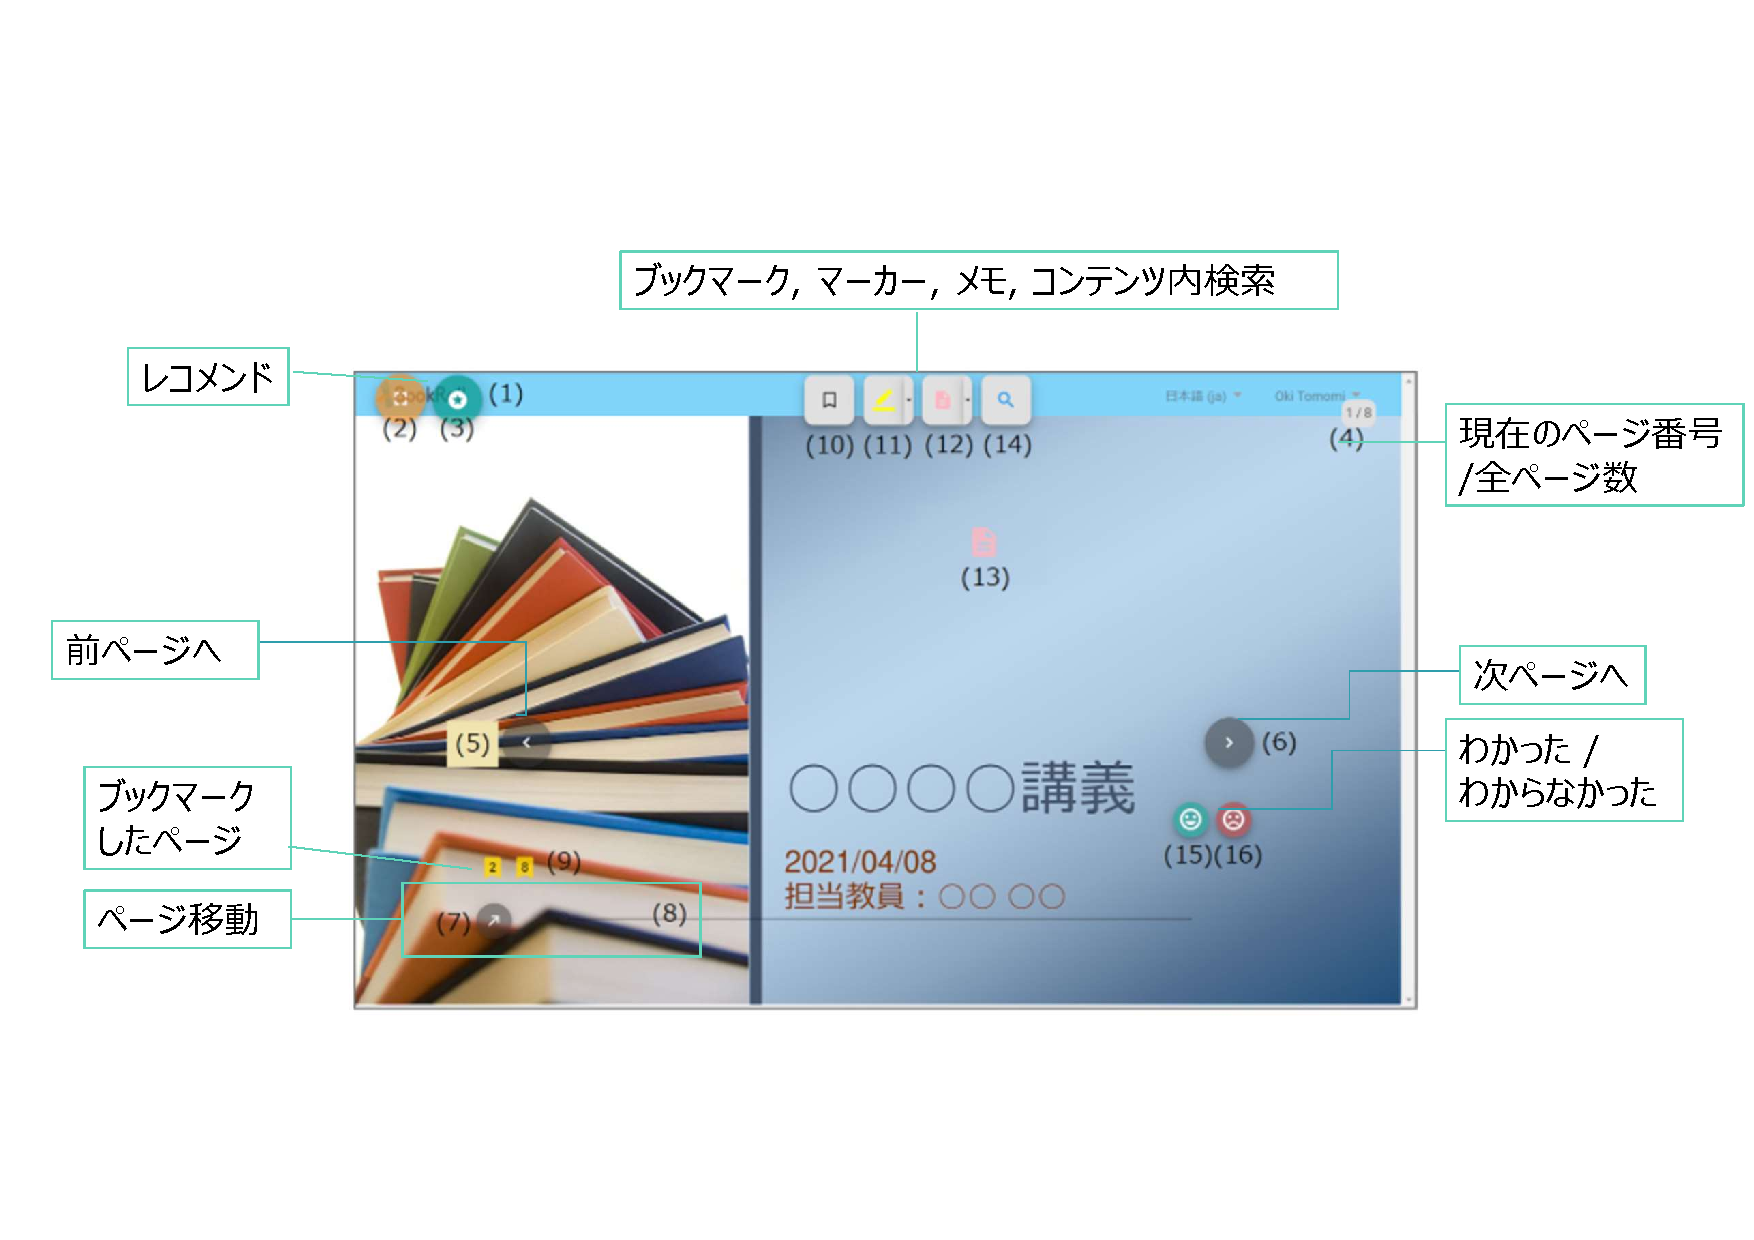
\includegraphics[scale = 0.4]{BookRoll.pdf}
  \vspace{-10mm}
  \caption{BookRoll コンテンツ閲覧画面例~\cite{BookRollgamen}}
  \label{fig:gamen}
\end{figure}


\begin{table}[tbp]
  \centering
  \caption{記録される主な内容}
  \label{tb:kirokunaiyou}
  \begin{tabular}{l|l}
    記録名 & 内容 \\ \hline
    contents\_id/name & コンテンツID/名 \\ 
    marker\_position/color & マーカーをつけた場所/色 \\ 
    memo\_title/text & メモのタイトル/内容 \\
    operation\_date/name & 操作した日時/操作内容 \\  
    page\_no & 操作したページ番号 \\ 
    userid & 学生に割り振られた番号 \\ \hline
  \end{tabular}
\end{table}

\begin{table}[tbp]
  \centering
  \caption{操作内容の一部}
  \label{tb:operationname}
  \begin{tabular}{l|l}
    操作名  (operation\_name)  & 内容 \\ \hline
    OPEN & コンテンツを開く \\ 
    CLOSE & コンテンツを閉じる \\ 
    NEXT & 次のページへ移動 \\
    PREV & ひとつ前のページへ移動 \\ 
    PAGE\_JUMP & 特定のページへ移動 \\ 
    ADD/DELETE BOOKMARK & ブックマークをつける/消す \\
    ADD/DELETE MARKER & マーカーをつける/消す \\
    ADD/DELETE/CHANGE MEMO & メモをつける/消す/変える \\ % 本当は「DELETE_MEMO」
    SEARCH & コンテンツ内検索を行う \\
    SEARCH\_JUMP & コンテンツ内検索結果のページに移動 \\
    GETIT & わかったボタンを押す \\ 
    NOTGETIT & わからなかったボタンを押す \\
    CLICK/OPEN/CLOSE\_RECOMMENDATION & 関連サイトをクリック/開く/閉じる \\ \hline
  \end{tabular}
\end{table}


\section{本研究の使用データ}\label{sec:data}

本研究では2020年に九州大学の情報系科目の講義で取得されたBookRollシステムの閲覧データ,講義で用いられたコンテンツ,および講義中に行われた小テストの結果(小テストデータ)を用いる.
講義は100名の学生に対し90分の講義が7週間に渡って行われ,各講義の最後の約10分間で小テストが行われた.講義から取得された閲覧データは計200,818行のログからなる.

7週の講義のうち,1週目と2週目では2つのコンテンツを使っている.1週目のコンテンツのうち1つはガイダンス資料であり,2週目はコンテンツに対応した小テストが2回行われている.

\section{閲覧データの記述統計量}\label{sec:toukei}
% 全然記述統計量でない場所もあるので名前変えたい

本節では,閲覧データから読み取ることのできる,各種操作の記述統計量を示し,その特徴について述べる.

% \noindent{\bf マーカーについて}\quad
\subsection*{マーカーについて}

表~\ref{tb:marker}はADD MARKERとDELETE MARKERの学生ごとの総操作回数の統計量,図~\ref{fig:add_marker},図~\ref{fig:delete_marker}はそれぞれの総操作回数の箱ひげ図である. 
% 図から,
表~\ref{tb:marker}より,よく使用している学生と使用していない学生にはかなり差がみられる.~\ref{sec:bookroll}節で述べた通り,色は3色用意されているが,色分けして使っている学生もいれば,色分けはせずに
% 記号的
目印的
に使っている学生もいる.
学生がマーカーのつけた場所を確認すると,多くのマーカーは学生が個人的につけているものであるが,ページによってはほとんどの学生がマーカーを付けている場所もあるため,教師の発言からマーカーを引いているページもあると考えられる.% あると言える (何を読み取れる) 信頼性がどのくらいなのか
% みられる->ひらがなで統一

\begin{table}[bp]
  \centering
  \caption{学生ごとのマーカーに関わる総操作回数の統計量}
  \label{tb:marker}
  \begin{tabular}{l||c|c}
    操作名 & ADD MARKER & DELETE MARKER \\ \hline\hline
    平均 & 19.37 & 1.74 \\ \hline
    標準偏差 & 39.41 & 5.28 \\ \hline
    最小値 & 0.00 & 0.00 \\ \hline
    第一四分位数 & 0.00 & 0.00 \\ \hline
    第二四分位数 & 5.50 & 0.00 \\ \hline
    第三四分位数 & 19.00 & 1.00 \\ \hline
    最大値 & 229.00 & 42.00 \\ \hline
  \end{tabular}
\end{table}


\begin{figure}[tbp]
  \begin{minipage}[b]{0.5\linewidth}
    \centering
    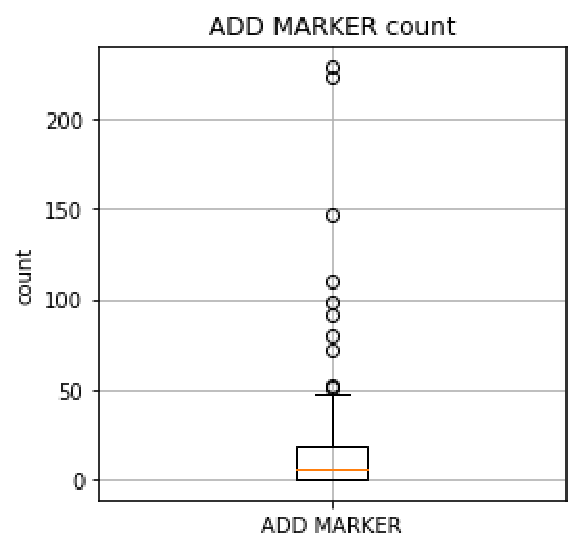
\includegraphics[scale=0.7]{add_marker.pdf}
    \caption{ADD MARKERの回数の箱ひげ図}
    \label{fig:add_marker}
  \end{minipage}
  \begin{minipage}[b]{0.5\linewidth}
    \centering
    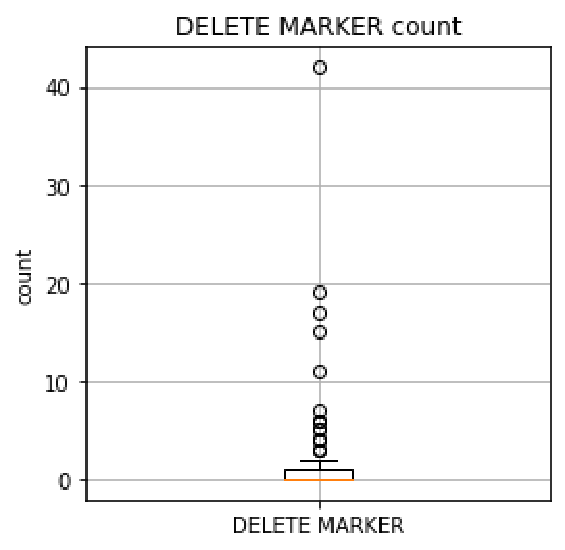
\includegraphics[scale=0.7]{delete_marker.pdf}
    \caption{DELETE MARKERの回数の箱ひげ図}
    \label{fig:delete_marker}
  \end{minipage}
\end{figure}

% \noindent{\bf GETIT,NOTGETITについて}\quad
\subsection*{GETIT,NOTGETITについて}

表~\ref{tb:get}はGETIT,NOTGETITの学生ごとの総操作回数の統計量である.
% GETIT,NOTGETIT共に,使用している人数に偏りがあることがわかる.
NOTGETITは使用している人数に偏りがあることがわかる.
% あまり使用されていないことがわかる.
% NOTGETITの記録数がすくないニュアンスがない
% 特にNOTGETITは記録されておらず,NOTGETITの方が記録が多いページは7ページのみである.
GETITと比べて,NOTGETITの記録数の方が顕著に少なく,NOTGETITの方が記録が多いページは7ページのみである.
表紙のような情報のないページでもGETIT,NOTGETITが記録されているコンテンツがあるため,どのテーマ,トピックがわからなかったかの目印として記録している学生がいるようにみえる.
% 箱ひげ図付録にいれる?

% コンテンツごとの記録数の表があってもいいかも

\begin{table}[tbp]
  \centering
  \caption{学生ごとの理解に関わる操作回数の統計量}
  \label{tb:get}
  \begin{tabular}{l||c|c}
    操作名 & GETIT & NOTGETIT \\ \hline\hline
    平均 & 119.23 & 12.05 \\ \hline
    標準偏差 & 128.32 & 17.95 \\ \hline
    最小値 & 0.00 & 0.00 \\ \hline
    第一四分位数 & 2.00 & 0.00 \\ \hline
    第二四分位数 & 70.50 & 5.00 \\ \hline
    第三四分位数 & 206.00 & 18.25 \\ \hline
    最大値 & 460.00 & 82.00 \\ \hline
  \end{tabular}
\end{table}

% \noindent{\bf メモについて}\quad
\subsection*{メモについて}

表~\ref{tb:memo}はADD MEMO,DELETE MEMO,CHANGE MEMOの学生ごとの総操作回数の統計量である.
表~\ref{tb:memo}より,メモはあまり使用されていおらず,使用している学生は偏りがあることがわかる.
% メモはタイトルと本文が同じタイミングで記録される.
% タイトルに本文を書いている学生もおり,
% タイトルと本文の両方が記録されているログは,7ログのみである.

\begin{table}[tbp]
  \centering
  \caption{学生ごとのメモに関わる操作回数の統計量}
  \label{tb:memo}
  \begin{tabular}{l||c|c|c}
    操作名 & ADD MEMO & DELETE MEMO & CHANGE MEMO \\ \hline\hline
    平均 & 1.06 & 0.12 & 0.24 \\ \hline
    標準偏差 & 4.08 & 0.41 & 1.00 \\ \hline
    最小値 & 0.00 & 0.00 & 0.00 \\ \hline
    第一四分位数 & 0.00 & 0.00 & 0.00 \\ \hline
    第二四分位数 & 0.00 & 0.00 & 0.00 \\ \hline
    第三四分位数 & 0.00 & 0.00 & 0.00\\ \hline
    最大値 & 33.00 & 2.00 & 7.00 \\ \hline
  \end{tabular}
\end{table}

% \noindent{\bf ブックマークについて}\quad
\subsection*{ブックマークについて}

表~\ref{tb:boookmark}はADD BOOKMARK,DELETE BOOKMARKの学生ごとの総操作回数の統計量,図~\ref{fig:addbookmark}はADD BOOKMARKの総操作回数の箱ひげ図である.
図~\ref{fig:addbookmark}より,BOOKMARKを使用している学生にかなり偏りがあることがわかる.
% 追加分
BOOKMARKを使用している学生は,BOOKMARKをつけたページからコンテンツを開くこともあり,復習のために使っているようにみえる.

\begin{table}[tbp]
  \centering
  \caption{学生ごとのブックマークに関わる操作回数の統計量}
  \label{tb:boookmark}
  \begin{tabular}{l||c|c}
    操作名 & ADD BOOKMARK & DELETE BOOKMARK \\ \hline\hline
    平均 & 1.72 & 0.25 \\ \hline
    標準偏差 & 7.76 & 0.97 \\ \hline
    最小値 & 0.00 & 0.00 \\ \hline
    第一四分位数 & 0.00 & 0.00 \\ \hline
    第二四分位数 & 0.00 & 0.00 \\ \hline
    第三四分位数 & 0.00 & 0.00 \\ \hline
    最大値 & 65.00 & 6.00 \\ \hline
  \end{tabular}
\end{table}

\begin{figure}[tbp]
  \centering
  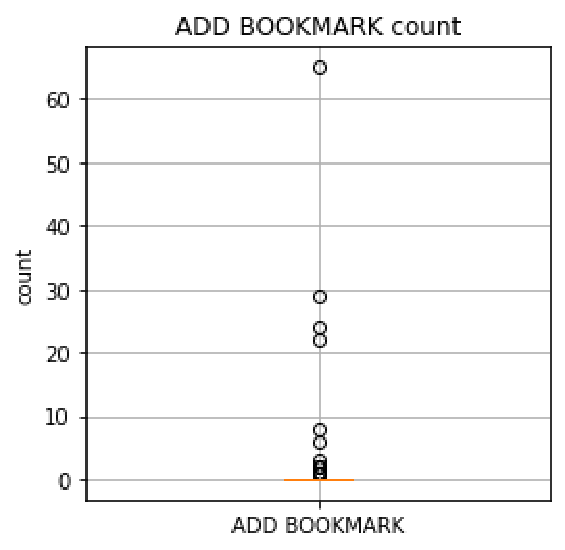
\includegraphics[scale = 0.7]{add_bookmark.pdf}
  \caption{ADD BOOKMARKの回数の箱ひげ図}
  \label{fig:addbookmark}
\end{figure}


\section{小テストデータの記述統計量}\label{sec:quiz}

~\ref{sec:data}節で述べた通り,小テストは毎週講義後に10分間で行われている.
小テストは5問の択一式の問題から成り,学生が小テストを提出したタイミングで,問題の文章,学生の選択した選択肢,正解か否か,および提出時間が記録される.
表~\ref{tb:scoredistribution}は各講義回ごとの点数の分布である.表より
% ~\ref{tb:scoredistribution}の要素は人数であり,
多くの学生が満点をとっているが,小テストによっては点数にばらつきがあることが確認できる.
講義に登録している学生は100名だが,
% 全ての講義,もしくは途中の講義から講義に参加しなくなった学生
全ての講義に参加していない学生,途中の講義から参加しなくなった学生,講義を休んだ回がある学生
がいるため,各小テストの分析は表~\ref{tb:scoredistribution}の合計人数で行っている.


% 全ての学生に対して小テストの問題文自体に変化ないが,学生ごとに正解文の書き方,解答の選択肢の順番が違っている.
出題される小テストの問題文は全ての学生に対して共通であるが,選択肢の一つである正解の文章や選択肢の順序は学生ごとに変化がつくようになっている.
具体的には正解文は数通り用意されているが,文意は基本的には同じである.
% 正解の文章は問題ごとに3つ用意されており,そのうち1つが正解として各学生の小テストに表示されている.3つの正解文に大きな違いは見られない.
% 小テストが2回分行われているため,提出時間にはかなり幅がある.
小テスト中もコンテンツの閲覧は許可されており,小テストの提出時間を確認すると,点数の低い人は提出時間が比較的早めであり,提出時間が遅くなるにつれて点数の高い人が増えているため,資料を確認しつつ答えている人がいることがわかる.
% 提出時間のグラフいれる?

% 以下のようなことが確認される→列挙
% 接続語や段落の切り替え
% 構造がわかりにくい

\begin{table}[tbp]
  \centering
  \caption{各小テストのスコア分布(人)}
  \label{tb:scoredistribution}
  \begin{tabular}{c||c|c|c|c|c|c|c|c}
    スコア & 1週目 & 2週目 & 2週目 & 3週目 & 4週目 & 5週目 & 6週目 & 7週目 \\
    (点) &  & (1) & (2) &  &  &  &  &  \\ \hline\hline
    0 & 0 & 0 & 0 & 0 & 0 & 0 & 0 & 1 \\ \hline
    1 & 1 & 1 & 0 & 0 & 1 & 1 & 2 & 3 \\ \hline
    2 & 3 & 1 & 0 & 0 & 1 & 2 & 5 & 6 \\\hline
    3 & 12 & 11 & 3 & 1 & 14 & 12 & 15 & 28 \\ \hline
    4 & 42 & 23 & 40 & 9 & 30 & 33 & 23 & 28 \\ \hline
    5 & 34 & 54 & 47 & 80 & 43 & 42 & 45 & 24 \\ \hline\hline
    合計人数 & 92 & 90 & 90 & 90 & 89 & 90 & 90 & 90 \\ \hline
  \end{tabular}
\end{table}


% \section{閲覧データとコンテンツ情報の分析}\label{sec:bunseki}

% 本節では閲覧データとコンテンツ情報について分析を行う.まず,コンテンツに含まれる各ページのテキスト情報をベクトル化し,ページ間の関係を観察する.続いて,操作された時間に注目し,いくつかの時間区分にわけて分析を行う.

% ページごとにもとめたページベクトル同士をコサイン類似度を用いて関係をみた.
% \subsection{コンテンツ情報の分析}
\section{コンテンツ情報の分析}\label{sec:bunseki}

本節では各コンテンツにおいてページ間の関係があるか分析する.ページ間の類似度を確認するためにページに含まれるテキスト情報のベクトル化を行い,各ページベクトルのコサイン類似度を求める.

ベクトル化には
% どのデータで事前学習?touhokuのやつを改めてっていう話をしよう!
事前学習済みのSentence-BERT~\cite{sonoisa} \footnote{日本語版BERTモデル~\cite{touhoku}を未公開のデータセットでMultipleNegativesRankingLossを用いてファインチューニングを行ったSentence-BERTモデル}を使用してコンテンツ${c}$に含まれるページ${p^{(c)}}$ごとに768次元の「ページベクトル」$\bm{v}_{(c,p)}$を求める.ただし単位ベクトルに正規化を行った.
コサイン類似度は対象となる2つのベクトルの距離を図る指標である.式(~\ref{cossim})で計算され,0-1で表現される.
\begin{align}\label{cossim}
  cos\_similarity (x,y)  = \frac{x \cdot y}{\parallel x \parallel \parallel y \parallel} = \frac{\sum_n {x_n}{y_n}}{\sqrt{\sum_n {x_n}^2+\epsilon} \sqrt{\sum_n {y_n}^2+\epsilon}}
\end{align}
式(~\ref{cossim})の分母に含まれる$\epsilon$は分母が0にならないための,0に近い整数である.
% 段落わけずにイプシロンの説明

図~\ref{fig:1cos}から図~\ref{fig:7cos}は各コンテンツにおけるページ間のコサイン類似度をヒートマップに表したものである.1に近いほど(ページ間の距離が近いほど)色が濃くなっている.
これらの図では,どのコンテンツにおいてもいくつかのページがひと固まりになっている部分があることがわかる.実際にコンテンツを確認してみると,コサイン類似度においてひと固まりとされているページ間はある程度同じトピックが説明されているため,
このページベクトルは各ページに含まれるテキスト情報をよく表現しているといえる.
% よく表現されているといえる.
しかし,コンテンツ自体が1つのテーマをもっているため,離れたページでも強く関係があるとされているページも存在する.
なお,コンテンツには図表を使用しているページもあるが,その図表に含まれる内容および位置関係についてはベクトル化を行っていない.

\begin{figure}[tbp]
  \begin{minipage}[b]{0.5\linewidth}
    \centering
    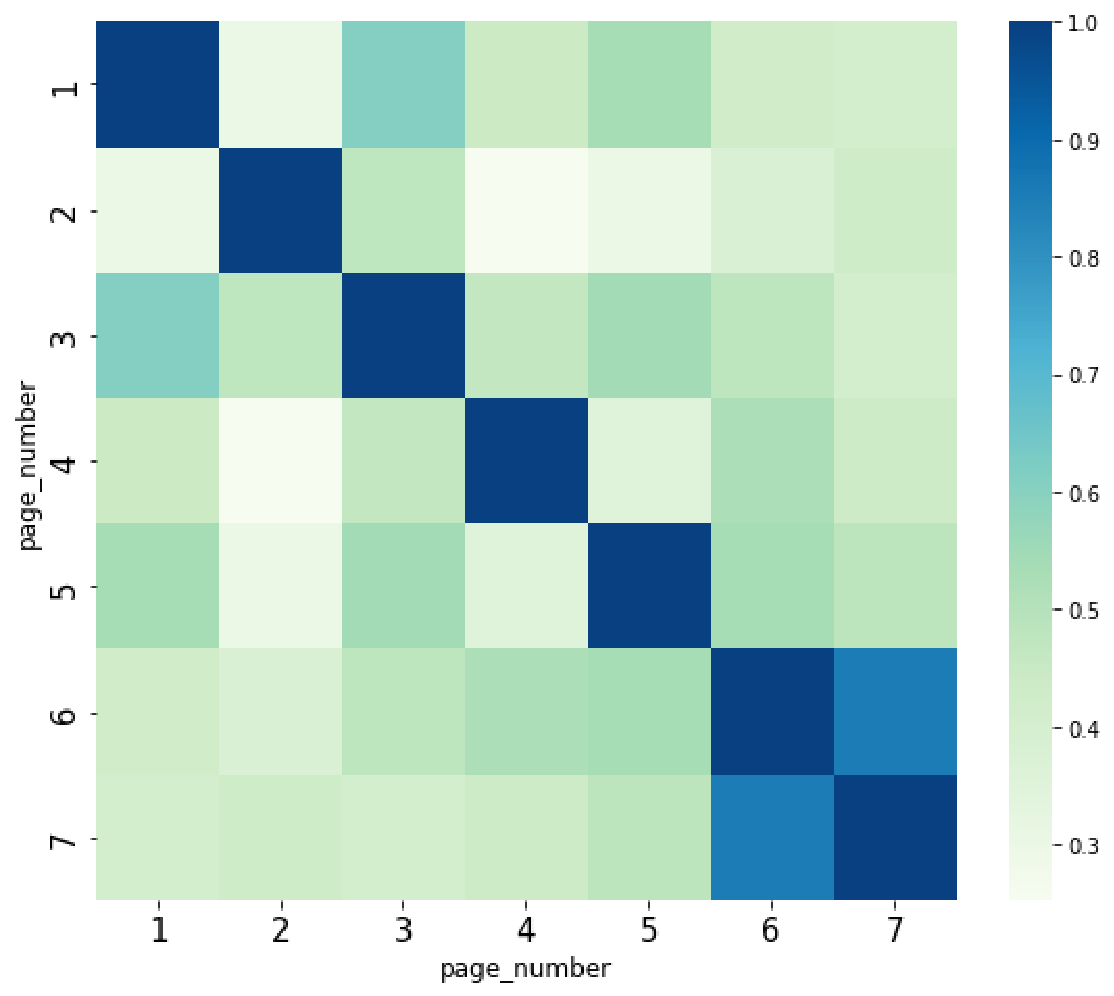
\includegraphics[scale=0.35]{1cos.pdf}
    \caption{各ページ間の類似度(1週目ガイダンス)}
    \label{fig:1cos}
  \end{minipage}
  \begin{minipage}[b]{0.5\linewidth}
    \centering
    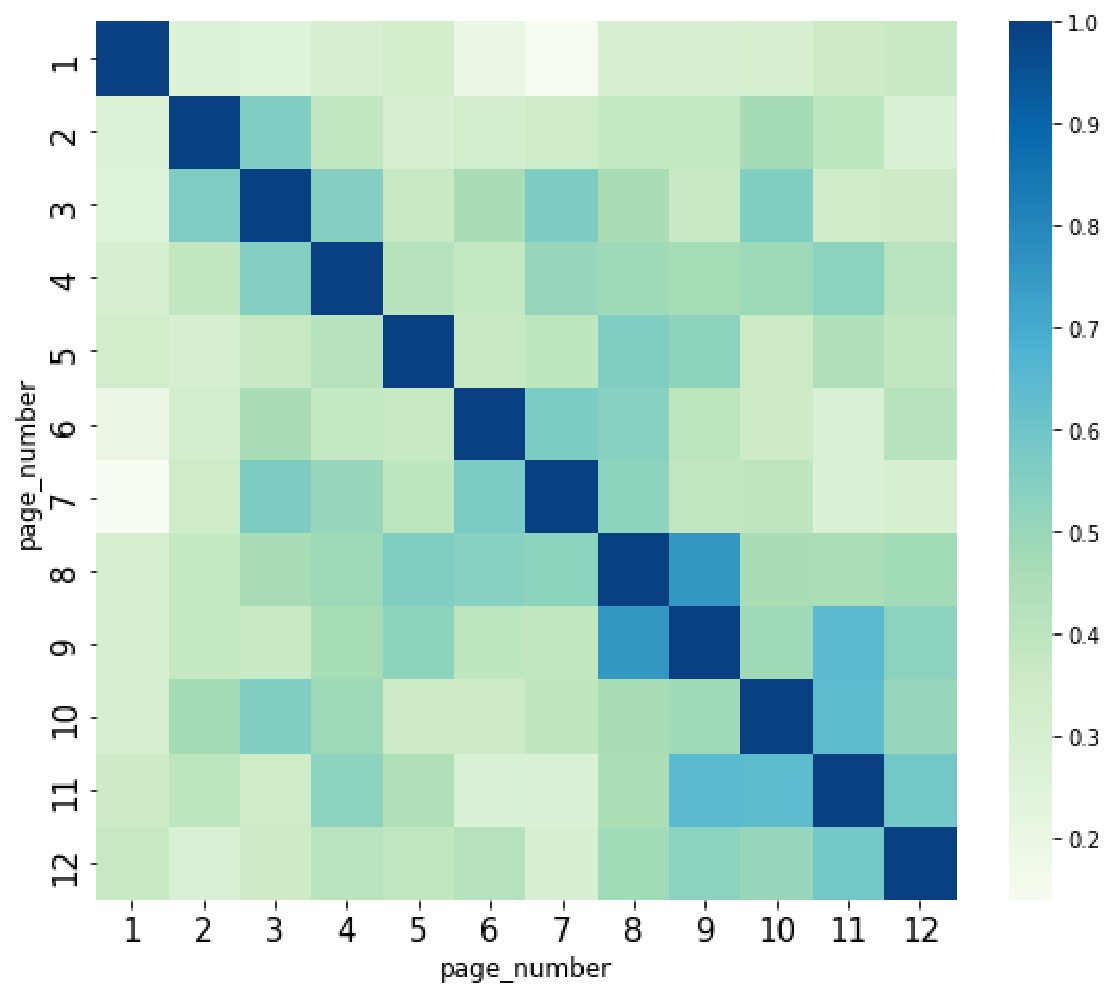
\includegraphics[scale=0.35]{1_cos.pdf}
    \caption{各ページ間の類似度(1週目講義資料)}
    \label{fig:1-cos}
  \end{minipage}
\end{figure}

\begin{figure}[tbp]
  \begin{minipage}[b]{0.5\linewidth}
    \centering
    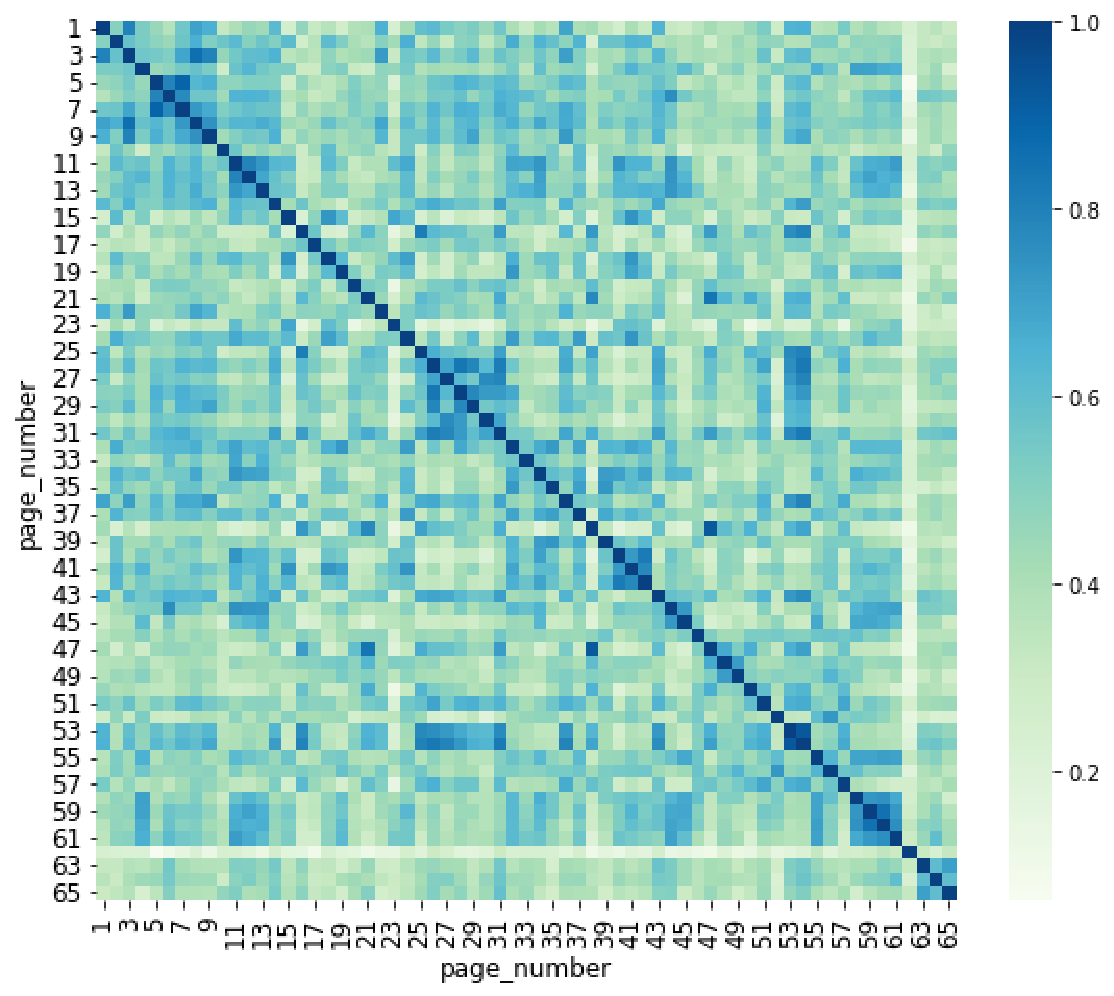
\includegraphics[scale=0.35]{2_1cos.pdf}
    \caption{各ページ間の類似度(2週目(1))}
    \label{fig:2-1cos}
  \end{minipage}
  \begin{minipage}[b]{0.5\linewidth}
    \centering
    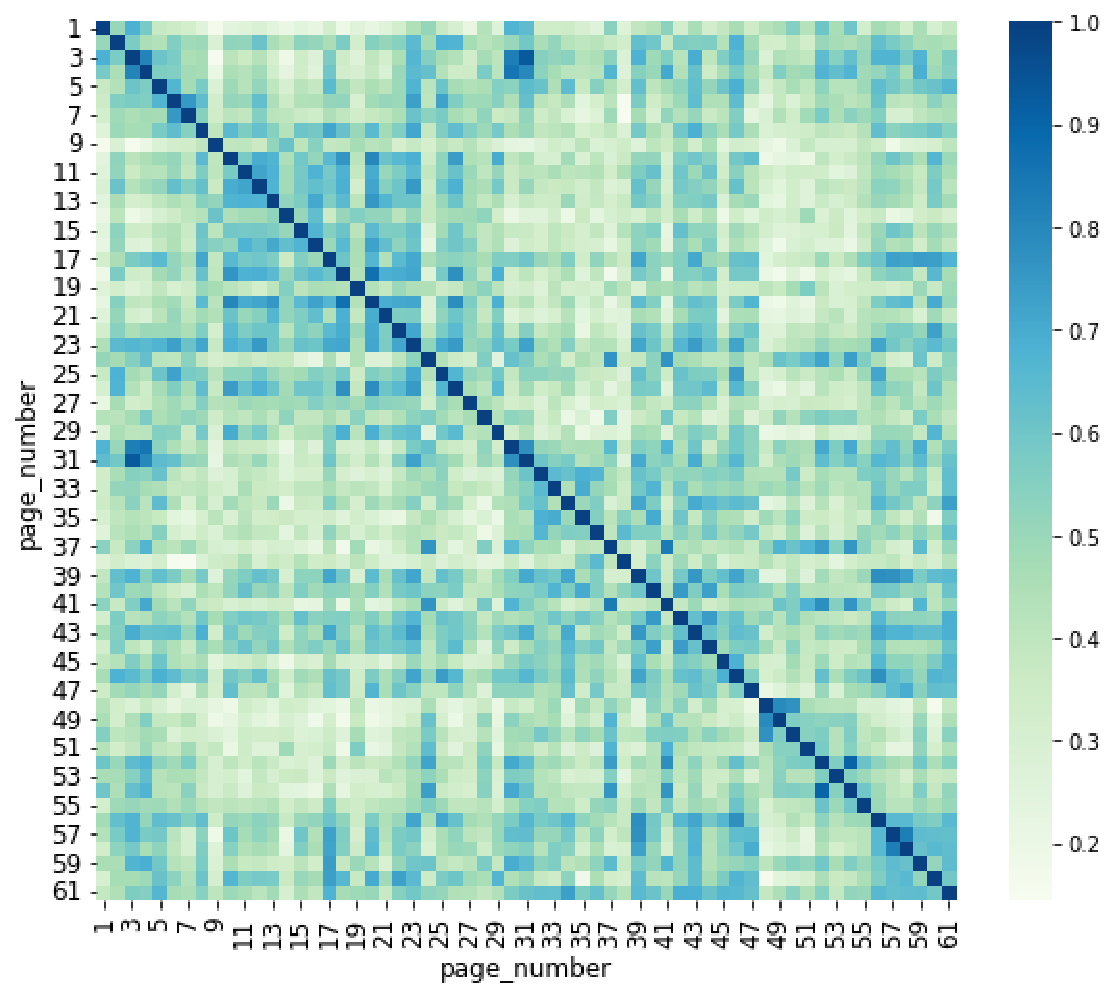
\includegraphics[scale=0.35]{2_2cos.pdf}
    \caption{各ページ間の類似度(2週目(2))}
    \label{fig:2-2cos}
  \end{minipage}
\end{figure}

\begin{figure}[tbp]
  \begin{minipage}[b]{0.5\linewidth}
    \centering
    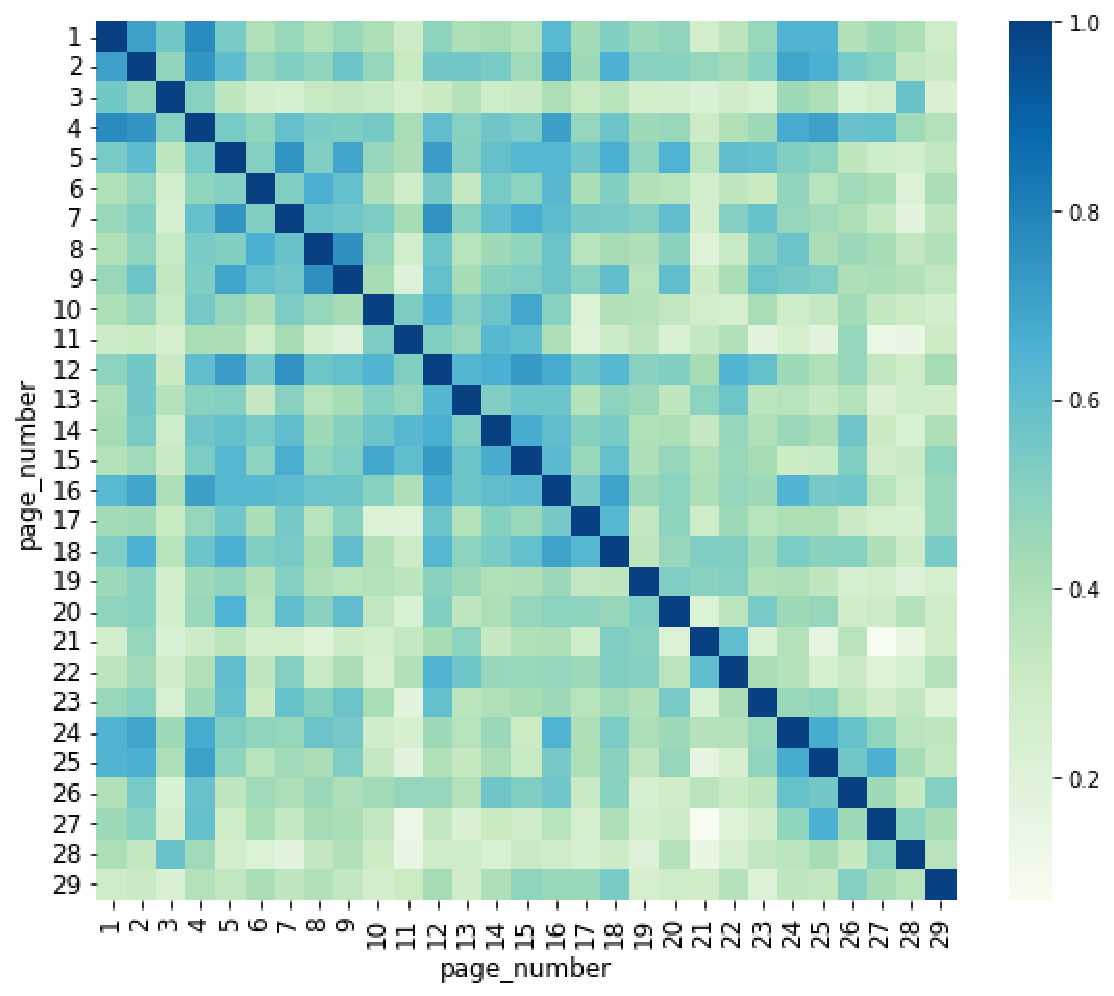
\includegraphics[scale=0.35]{3cos.pdf}
    \caption{各ページ間の類似度(3週目)}
    \label{fig:3cos}
  \end{minipage}
  \begin{minipage}[b]{0.5\linewidth}
    \centering
    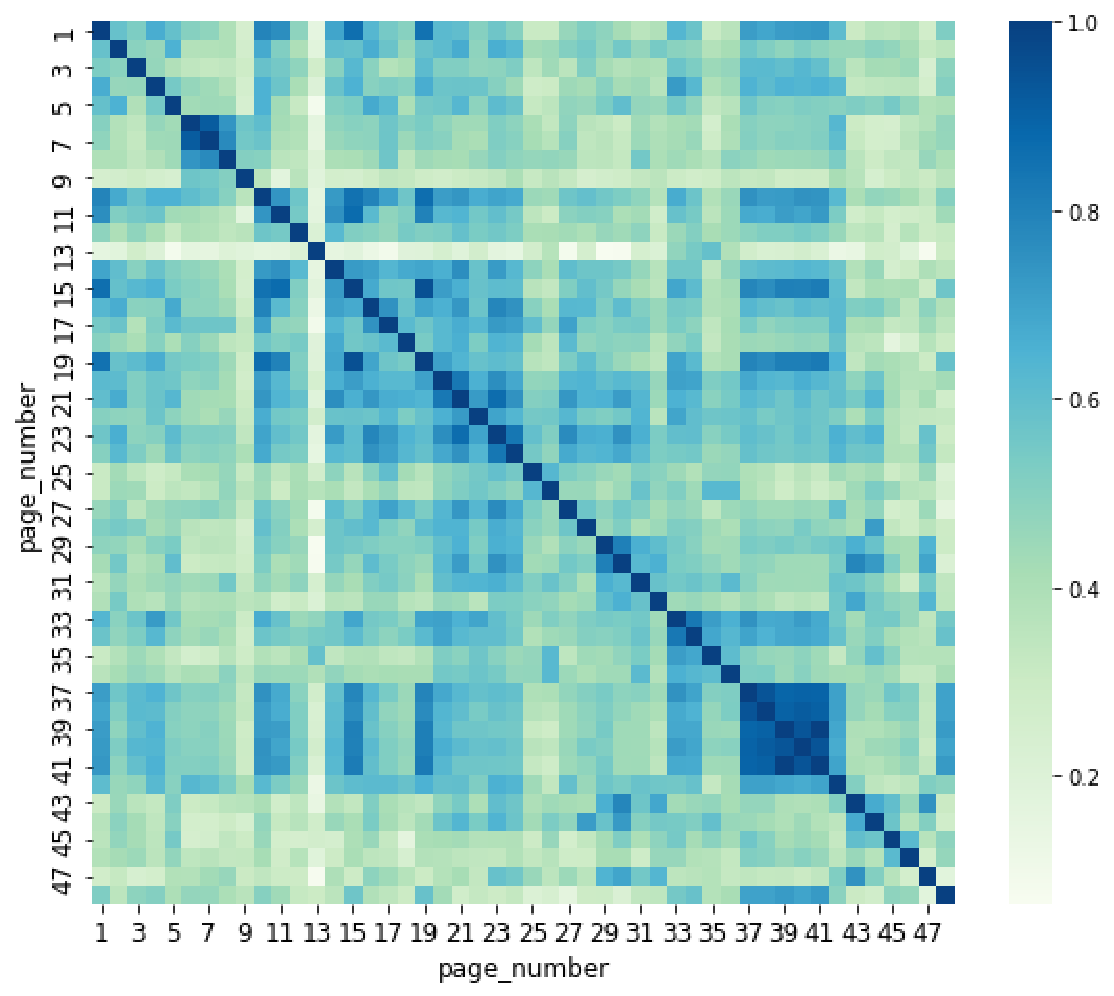
\includegraphics[scale=0.35]{4cos.pdf}
    \caption{各ページ間の類似度(4週目)}
    \label{fig:4cos}
  \end{minipage}
\end{figure}

\begin{figure}[tbp]
  \begin{minipage}[b]{0.5\linewidth}
    \centering
    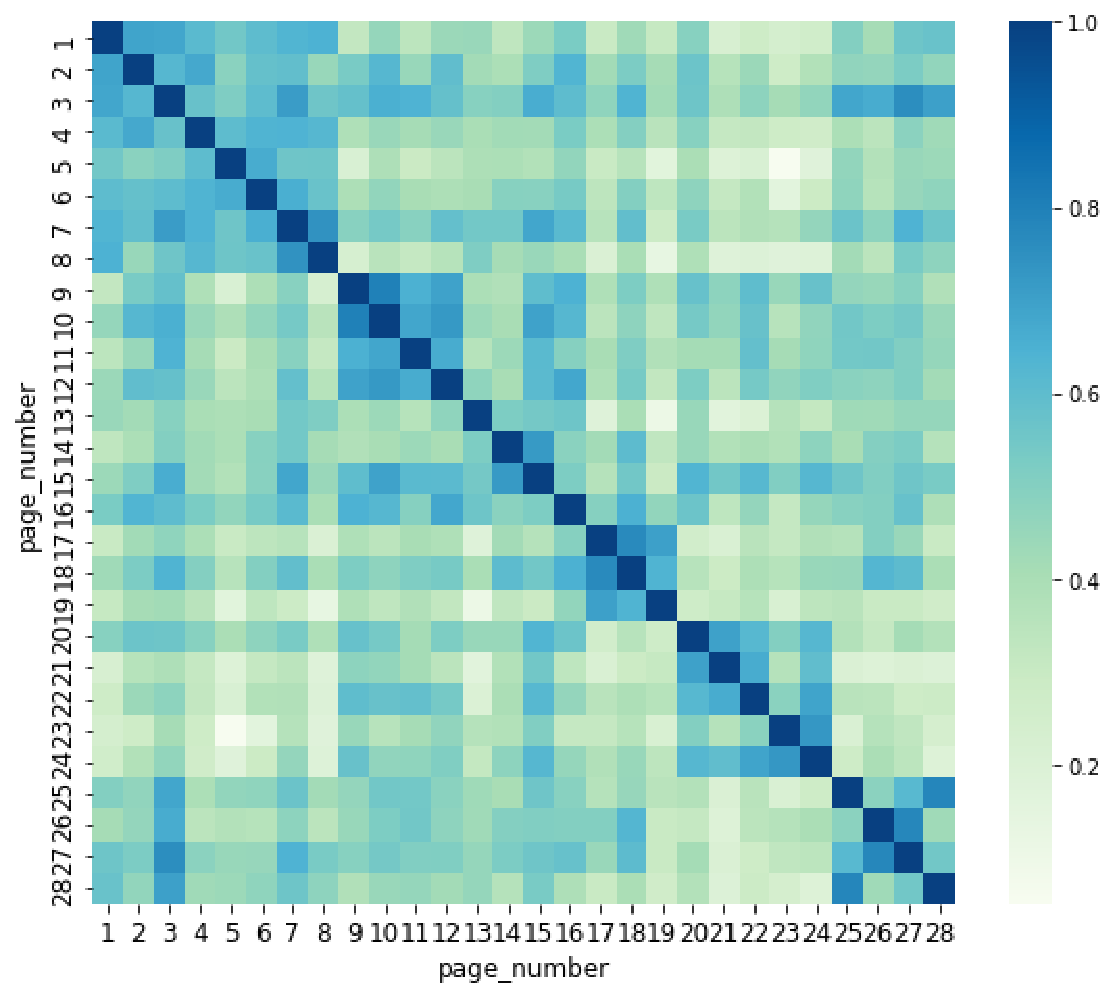
\includegraphics[scale=0.35]{5cos.pdf}
    \caption{各ページ間の類似度(5週目)}
    \label{fig:5cos}
  \end{minipage}
  \begin{minipage}[b]{0.5\linewidth}
    \centering
    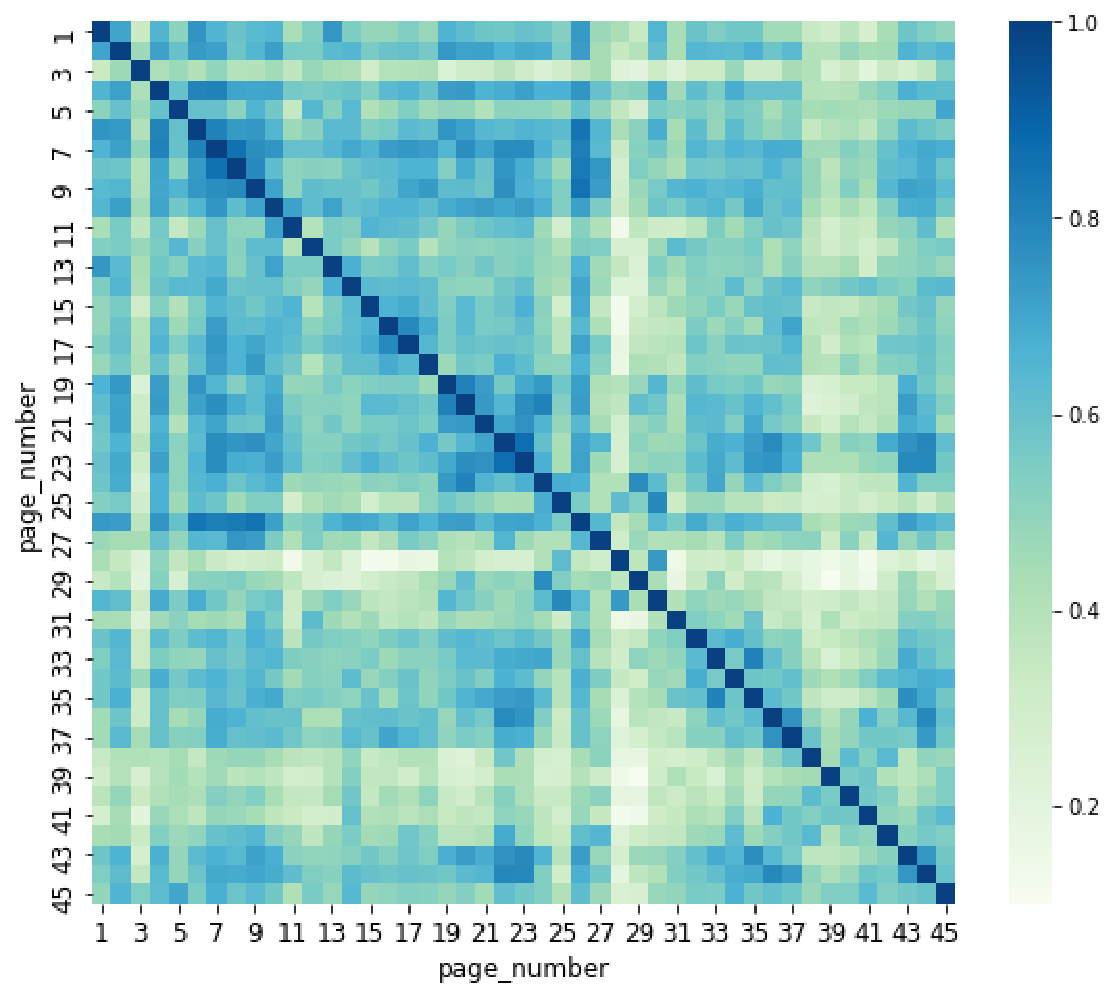
\includegraphics[scale=0.35]{6cos.pdf}
    \caption{各ページ間の類似度(6週目)}
    \label{fig:6cos}
  \end{minipage}
\end{figure}

\begin{figure}[tbp]
  \centering
  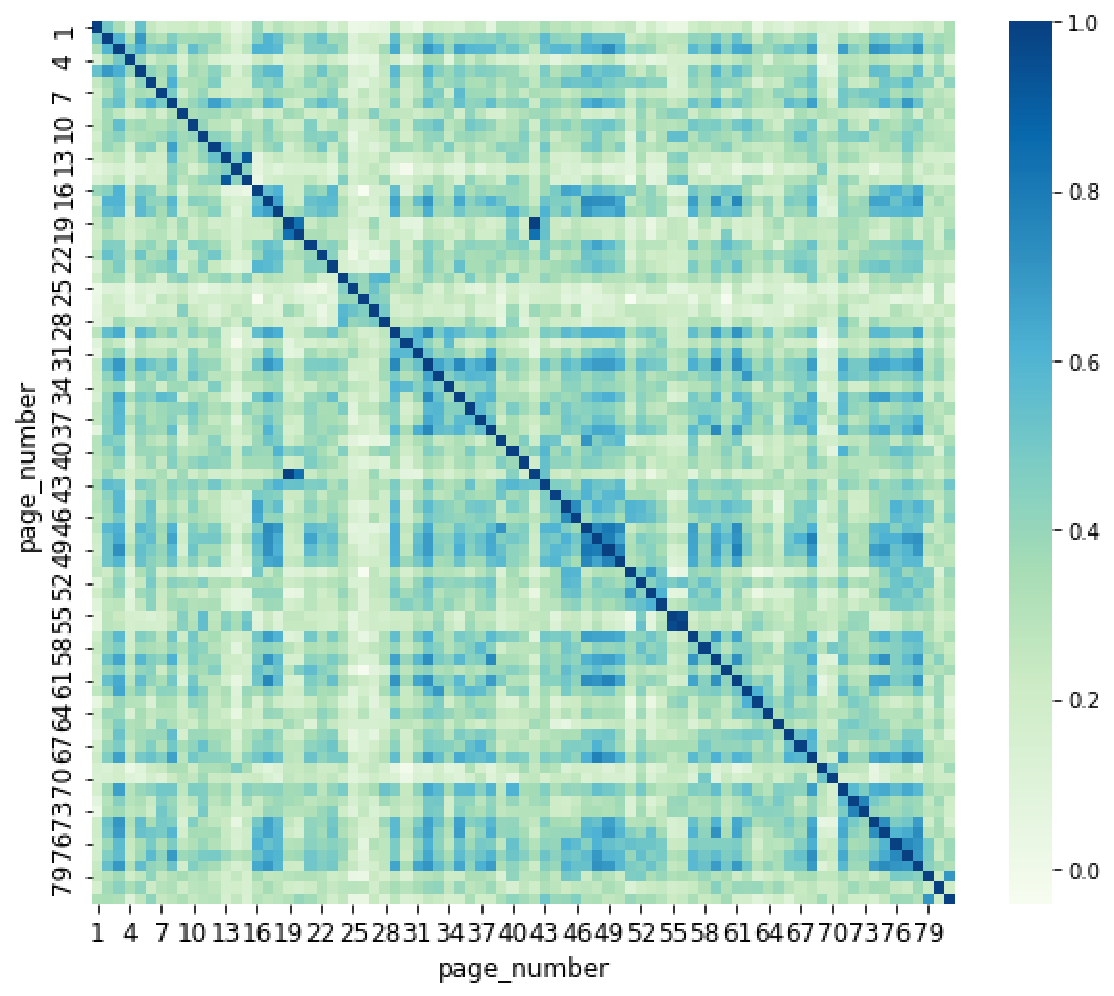
\includegraphics[scale=0.35]{7cos.pdf}
  \caption{各ページ間の類似度(7週目)}
  \label{fig:7cos}
\end{figure}


% \subsection{時間区分ごとの行動}
\section{時間区分ごとの行動分析}

本節では操作された時間に注目し,いくつかの時間区分にわけて分析を行う.
% 学生の行動がされた
学生が行動した
時間を講義時間内(inlec),小テスト時間内(intest),講義時間外(outlec)に分割し,分析を行った.
% 講義時間外の行動は特に講義時間前後1時間以内に行われているため,.
講義時間内,小テスト時間内,講義時間外で学生の総操作回数の10分ごとの時間平均をとった結果が表~\ref{tb:sousakaisuu}であり,
平均総操作回数が一番多い時間は小テスト時間内である.
なお講義時間外の範囲は,
全ての講義終了後1週間までとし,対象となる講義の予習復習のために活動可能な時間を各週1時間30分として時間平均を計算している.

ここで,時間区分ごとの行動をk-means法(k = 4)でクラスタリングを行った.その結果「全体的に活動にしている学生」「全体的に活動していない学生」「テスト時間中によく活動している学生」「全体的に活動量が多くもなく,少なくもない学生」というクラスタに分かれた.各クラスタの時間区分ごとの総行動数の箱ひげ図を図~\ref{fig:cluster}に示す.
% 「全体的に活動はしているが活動量が多くはない学生」
% 「全体的に活動量が中途半端な学生」
% 最も学生の多いクラスタは「全体的に活動量が中途半端な学生」のクラスタであり,44人がこのクラスタに分類されている.
最も学生の多いクラスタは「全体的に活動量が多くもなく,少なくもない学生」のクラスタであり,44人がこのクラスタに分類されている.
さらに,講義時間内,小テスト時間内,講義時間外を各講義単位に分割すると「全体的に活動はしているが多くはない学生」は前半から中頃にかけて活動が減り,後半にかけて活動が増えていることがわかった.

\begin{table}[tbp]
  \centering
  \caption{時間区分ごとの統計量}
  \label{tb:sousakaisuu}
  \begin{tabular}{c|c|c|c}
    & 講義時間内 & 小テスト時間内 & 講義時間外 \\ \hline\hline
    平均 & 18.17 & 33.64 & 11.83 \\ \hline
    標準偏差 & 10.58 & 29.54 & 10.67 \\ \hline
    最小値 & 0.00 & 0.00 & 0.00 \\ \hline
    第一四分位数 & 12.37 & 9.79 & 3.42 \\ \hline
    第二四分位数 & 16.78 & 24.21 & 9.32 \\ \hline
    第三四分位数 & 23.26 & 48.93 & 17.29 \\ \hline
    最大値 & 57.43 & 128.00 & 63.54 \\ \hline
  \end{tabular}
\end{table}

% \begin{figure}[tbp]
%   \centering
%   \includegraphics[scale = 0.4]{cluster.png}
%   \caption{各クラスタの時間区分ごとの総操作回数の箱ひげ図}
%   \label{fig:cluster}
% \end{figure}

\begin{figure}[tbp]
  \begin{minipage}[b]{0.32\linewidth}
    \centering
    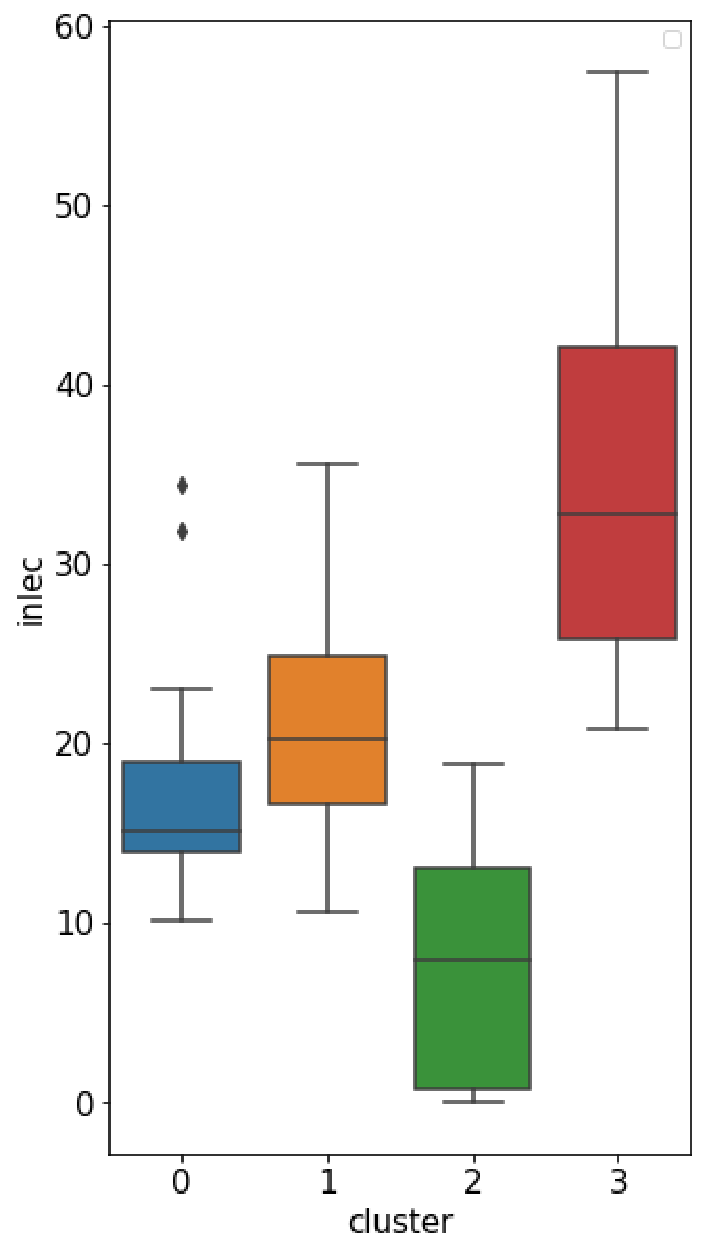
\includegraphics[keepaspectratio, scale=0.35]{inlec.pdf}
    \subcaption{講義時間内}
    \label{fig:inlec}
  \end{minipage}
  \begin{minipage}[b]{0.32\linewidth}
    \centering
    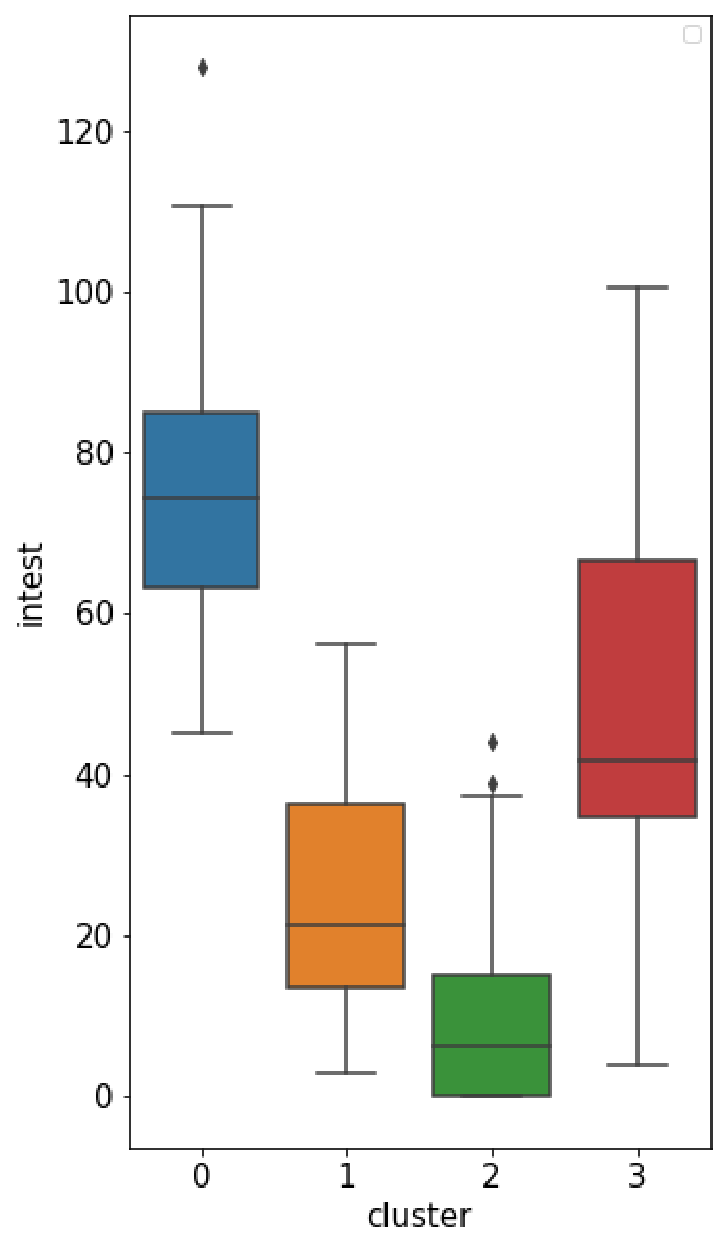
\includegraphics[keepaspectratio, scale=0.35]{intest.pdf}
    \subcaption{小テスト時間内}
    \label{fig:intest}
  \end{minipage}
  \begin{minipage}[b]{0.32\linewidth}
    \centering
    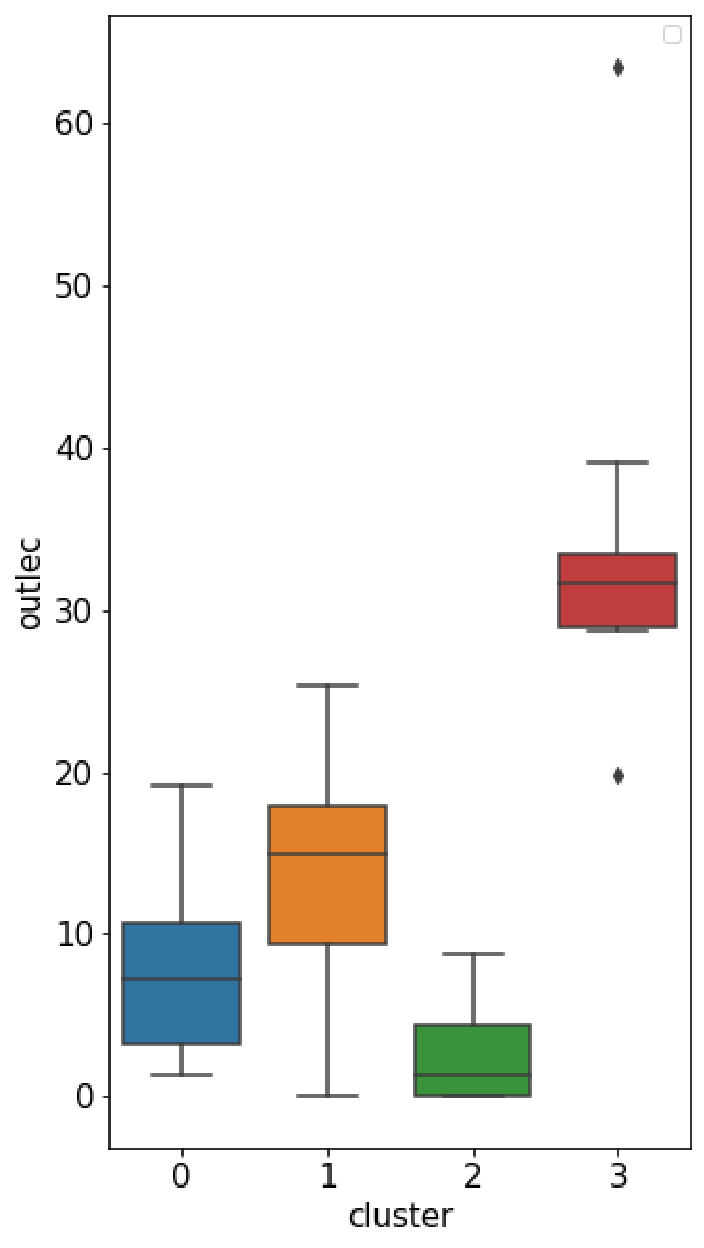
\includegraphics[keepaspectratio, scale=0.35]{outlec.pdf}
    \subcaption{講義時間外}
    \label{fig:outlec}
  \end{minipage}
  \caption{各クラスタの時間区分ごとの総操作回数の箱ひげ図}
  \label{fig:cluster}
\end{figure}


% 統計量の根拠となる内容を示そうね

% 標準化→最後に標準偏差かけて平均たす


% タイトルと同じ?
\chapter{学習者のスコア予測}

図~\ref{fig:overview}に本研究の全体像を示す.
本研究では学生の行動からスコア予測を行うベースラインに加えて,講義で使用されたコンテンツの情報を用いて学習者のスコア予測を行う.コンテンツ情報を用いてスコア予測を行うアプローチとして,学生が長く閲覧したコンテンツに含まれるテキスト情報を使用する手法1と小テストに関係するページの情報を使用する手法2を提案する.
% コンテンツ情報を使うことがポイント
% ~~~な手法1と~~~な手法2を提案する

\section{行動特徴ベクトルとコンテンツ情報を用いたスコア予測(提案手法1)}\label{sec:1}

% 要するにこういう考え方の手法だよ
% 1つ目の手法は学生の行動に加えてコンテンツに含まれるテキスト情報を使用する手法である.
% 提案手法1では学生の行動に加えてコンテンツに含まれるテキスト情報を使用する.
提案手法1では,学生の行動から得られる特徴ベクトルと,その学生が長く閲覧したコンテンツから得られる特徴ベクトルを連結して,スコア予測の特徴ベクトルとして用いる.

まず,BookRollから得られた閲覧データより,各学生について,あるコンテンツの各ページにおける操作タイプごとの操作回数および閲覧時間を求め,これらの特徴量を要素とするようなベクトルを各学生の「行動特徴ベクトル」と呼ぶ.
ここで,学生$i$のコンテンツ$c$における行動特徴ベクトルを$\bm{u}^{(i)}_c$と表す.
行動特徴ベクトル$\bm{u}^{(i)}_c$の次元数は「ページ数 $\times$(操作タイプ数 + 1)」(最後の1はページ閲覧時間に対応)であり,ページ数はコンテンツ$c$によりそれぞれ異なる.
ページ数は付録の表~\ref{tb:topic}に示す.
% 本研究では求めた行動特徴ベクトルを使用して2つのスコア予測手法を提案する.
% い,2つの手法と予測精度を比較する.

\begin{figure}[tbp]
  \centering
  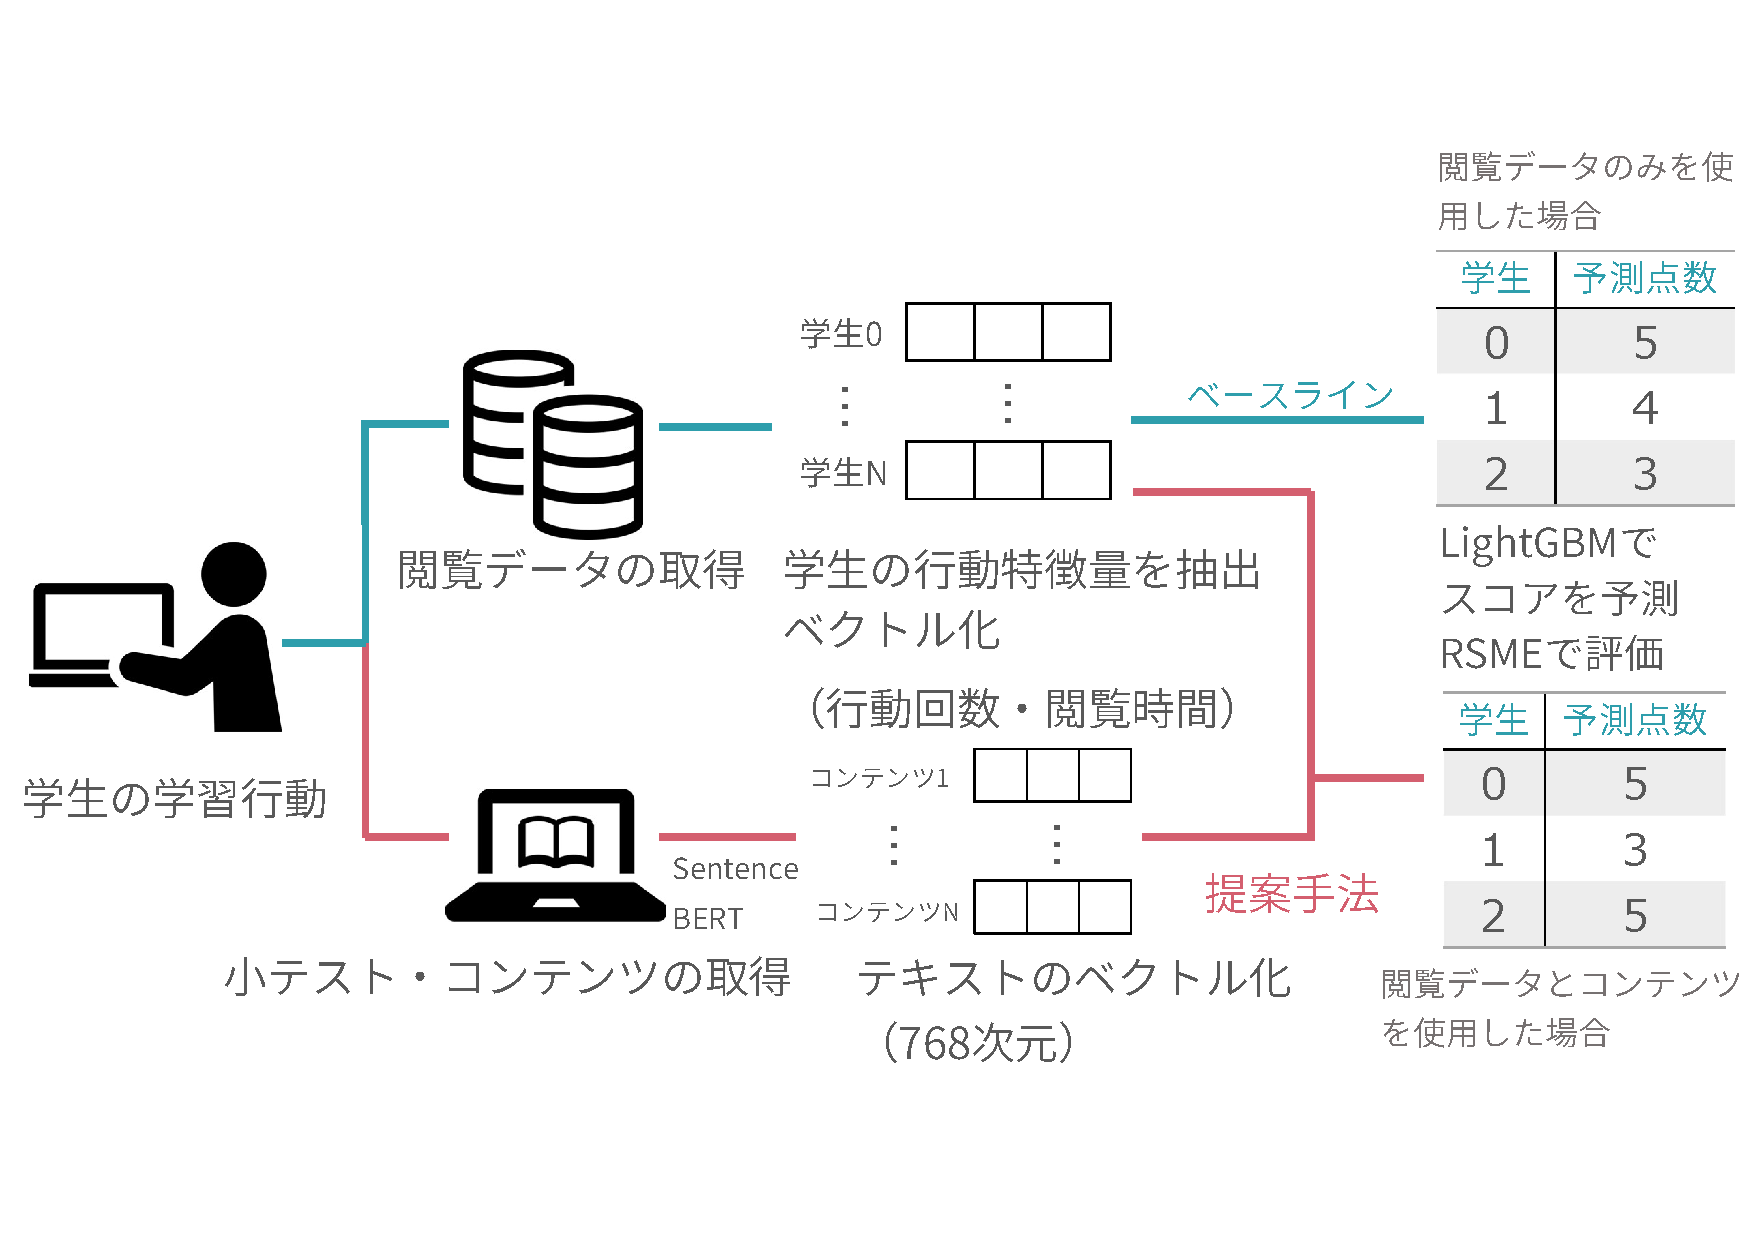
\includegraphics[scale = 0.4]{zentaizo2n.pdf}
  % \vspace{-5mm}
  \caption{本研究の全体像}
  \label{fig:overview}
\end{figure}


% 1つ目の提案手法はコンテンツ${c}$に含まれる文章のベクトル化を行い,そのベクトルを行動特徴ベクトルに連結してスコア予測を行う方法である.
次に,コンテンツ${c}$に含まれる文章のベクトル化を行い,そのベクトルを行動特徴ベクトルに連結してスコア予測を行う.
% ベクトル化に事前学習済みのSentence-BERT~\cite{sonoisa}を使用してページ${p^{(c)}}$ごとに768次元の「ページベクトル」$\bm{v}_{(c,p)}$を求める.ただし単位ベクトルに正規化を行った.
コンテンツに含まれる文章のベクトルには~\ref{sec:bunseki}節のページベクトル$\bm{v}_{(c,p)}$を使用する.
ページベクトルをそのまま連結すると全ての学生が同じページベクトルをもつことになるため,重みづけをすることで学生ごとに違ったベクトルを作成する.本研究では各ページの閲覧時間に注目し,学生$i$がコンテンツ$c$において長く閲覧したページの内容情報を多く含む「閲覧コンテンツベクトル」$\bm{v}^{(i)}_c$を,
% 求め,
% 各学生がよく閲覧したページの内容情報を多く含むようなベクトルを得るために,
学生$i$のページ$p$に対する閲覧時間の総和$t^{(i)}_{(c,p)}$に基づいてページベクトルに重みづけを行って足し合わせることで求める.具体的には,閲覧時間をそのまま各ページの重み $w^{(i)}_{(c,p)} = t^{(i)}_{(c,p)}$としてページベクトルの線形和 $\bm{v}^{(i)}_c = \sum_p w^{(i)}_{(c,p)}\bm{v}_{(c,p)}$ を求め,単位ベクトルに正規化して閲覧コンテンツベクトルとする.
ただし,同じページを継続して5分より長く開いていたログは,長時間放置されたものとして,各ページの閲覧時間の総和から除外した.

% 求めた閲覧コンテンツベクトル$\bm{v}^{(i)}_c$とページベクトル$\bm{v}^{(i)}_c$を連結させたベクトル$\bm{f}_{1, c}^{(i)} = (\bm{u}_{c}^{(i)}, \bm{v}_{c}^{(i)})$で予測を行う.
求めた行動特徴ベクトル$\bm{u}^{(i)}_c$と閲覧コンテンツベクトル$\bm{v}^{(i)}_c$を連結させ,以下の新たなベクトルを得る.

\begin{equation}
\bm{f}_{1, c}^{(i)} = (\bm{u}_{c}^{(i)}, \bm{v}_{c}^{(i)})
\end{equation}

提案手法1ではこの特徴ベクトル$\bm{f}_{1, c}^{(i)}$を用いてスコア予測を行う.

% 本研究では,さらに学生$i$がコンテンツ$c$においてよく閲覧したページの内容情報を多く含む「閲覧コンテンツベクトル」$\bm{v}^{(i)}_c$を求め,行動特徴ベクトルに連結する.この統合された特徴ベクトルを用いて,小テストのスコア予測を行う方法を提案する.

% ページベクトルは各ページに対し作成されているため,このままでは行動特徴量が大きくなるので,重みづけを行ったページベクトルをコンテンツごとに足し合わせることでベクトルの圧縮を行う.


% 小テストとの関連度 (による重みづけ) を用いた/に基づく成績予測
% 小テストに関わるコンテンツ
\section{小テストに関係するページを使用したスコア予測(提案手法2)}\label{sec:2}

% 2つ目の提案手法は,小テストに関係するページにおける行動をとりだしてスコア予測を行う方法である.
提案手法2では,小テスに関係するページにおける行動をとりだしてスコア予測を行う.
小テスト$q$に含まれる問題$j$ごとに,
% ,~\ref{sec:bunseki}節で述べたSentence-BERTにより
% 問題文と正解文をベクトル化し,
問題文と複数存在する正解文をすべてベクトル化し,
「小テストベクトル」$\bm{Q}_{(q,j)}$を作成する.
ここで,テキストのベクトル化には~\ref{sec:bunseki}節で述べたSentence-BERTに基づく手法を用いる.さらに,小テストベクトルとページベクトルの関係をみるために~\ref{sec:bunseki}節で用いた,コサイン類似度を使用する.
% 小テストベクトル$\bm{Q}_{(q,j)}$とページベクトル$\bm{v}_{(c,p)}$とのコサイン類似度を求め,各ページと各問とのコサイン類似度$cos\_similarity (\bim{Q}_{(q,j)}, \bim{v}_{(c,p)}) $が0.4以上のコサイン類似度の値の和を求め,各ページの重み$w^{(i)}_{(c,p)} = \sum_p cos\_similarity (\bim{Q}_{(q,j)}, \bim{v}_{(c,p)}) >0.4$とする.
% この重みを使って対応するページの行動特徴ベクトルに重みづけを行い,新たな行動特徴ベクトルとし,これを用いてスコア予測を行う.


コンテンツ$c$に対応する小テストを$q(c)$とする.このとき,コンテンツ$c$の各ページベクトル$\bm{v}_{(c,p)}$について,$q(c)$に含まれる5つの小問から得られる小テストベクトル$\bm{Q}_{(q(c),j)} \quad (j=1,...,5)$それぞれとのコサイン類似度を求め,その類似度の和をページ$p$の重み$w_{(c,p)}$とする.ただし,コサイン類似度が0.4未満である場合は和に含めないものとする.すなわち,重みは以下のように求める.
\begin{equation}
w_{(c,p)} = \sum_{j \in \mathcal{J}} cos\_similarity(\bm{Q}_{(q(c),j)}, \bm{v}_{(c,p)}) \\
\end{equation}
ただし,$\mathcal{J} = \left\{j \,|\, cos\_similarity(\bm{Q}_{(q(c),j)}, \bm{v}_{(c,p)}) \geq 0.4\right\}$である.

% (メモ:$w$に上付きの$(i)$は不要)

$w_{(c,p)}$は,各ページ$p$がどの程度小テスト$q(c)$に関連するかを表す重みであり,ページごとの行動特徴ベクトル$\bm{u}_{(c,p)}^{(i)}$をこの$w_{(c,p)}$で重みづけることにより,以下の新たな行動特徴ベクトルを得る.
\begin{equation}
\bm{f}_{2, c}^{(i)} = \sum_p w_{(c,p)} \bm{u}_{(c,p)}^{(i)}
\end{equation}
提案手法2ではをこの特徴ベクトル$\bm{f}_{2, c}^{(i)}$を用いてスコア予測を行う.


% 審議値(False,True)をたしているでとても腑に落ちました
% 手法1との違いを2文目くらいで書いてもいいかも?
% 手法1ではコンテンツベクトルに重みづけを行い,コンテンツベクトルを用いて予測を行うが,手法2では閲覧コンテンツベクトルに重みづけを行い,コンテンツベクトルは使用しない.


\chapter{評価}

\section{予測および評価方法}\label{sec:yosoku}

スコア予測は小テストごとにLightGBMを使用して行う.
LightGBMは勾配ブースティングに基づく機械学習手法である.高い予測精度で計算時間が速い点と,予測時に結果への寄与度が要素ごとにわかる点からLightGBMを使用した.
5-fold交差検証を用いて各foldのRSME (Root Mean Square Error)を計算し,各RMSEの平均により評価する.
評価には小テストごとに求めた学生のスコアを使用する.~\ref{sec:toukei}節で述べたように,2週目は2つのコンテンツが使用され,小テストが2回分行われたため,2週目(1)と2週目(2)に分けてスコア予測を行うものとする.

% しかし,このままの状態で行動特徴ベクトルを求めると,
行動特徴ベクトルとして,全ての操作タイプを用いた場合,ベクトルが大きくなりすぎてしまうため,
% 圧縮のために行動特徴ベクトルに含める操作タイプを一部除いた.
行動特徴ベクトルに含める操作タイプを限定した.
事前にLightGBMで全ての小テストの合計値のスコア予測を行った際に,予測結果への寄与度(Importance)が0であった操作タイプを除いた.
その結果,ここで用いる行動特徴ベクトルに含める操作タイプは,表~\ref{tb:Importance}に示す12タイプとなった.これに,ページの閲覧時間(open\_time)を加えた13次元の行動を実験では用いた.


行動特徴ベクトルは,講義時間外の操作を全て用いる場合と,講義時間内および前後1時間の操作に絞った場合の2通りで計算し比較する.
% ~\ref{sec:bunseki}節で述べた通り,
講義時間外の行動は特に講義時間内および前後1時間に偏りがあり,かつ本研究の目的の1つである,早めの学生へのレスポンスに繋がると考えるため,講義時間内および前後1時間の場合でもスコア予測を行う.

% 行動特徴ベクトルは,講義時間外の操作を全て用いる場合  (all)  と,講義時間内および前後1時間の操作に絞った場合  (in-lec)  の2通りで計算し比較する.
% ~\ref{sec:bunseki}節で述べた通り,講義時間外の行動は特に講義時間内および前後1時間に偏りがある,かつ本研究の目的の1つである,早めの学生へのレスポンスに繋がると考えたため,講義時間内および前後1時間の場合でもスコア予測を行う.

% ハイパーパラメータ、シャッフルなし


\begin{table}[tbp]
  \centering
  \caption{講義時間外含む}
  \label{tb:Importance}
  \begin{tabular}{l|c}
    操作名 & 予測結果への寄与度(Importance) \\ \hline\hline
    OPEN & 10.24 \\ \hline
    NEXT & 42.92 \\ \hline
    PREV & 78.11 \\ \hline
    CLOSE & 34.41 \\ \hline
    PAGE\_JUMP & 76.88 \\ \hline
    GETIT & 4.80 \\ \hline
    NOTGETIT & 5.76 \\ \hline
    OPEN\_RECOMMENDATION & 32.00 \\ \hline
    CLOSE\_RECOMMENDATION & 20.67 \\ \hline
    ADD MARKER & 4.27 \\ \hline
    DELETE MARKER & 1.80 \\ \hline
    CLICK\_RECOMMENDATION & 0.86 \\ \hline
  \end{tabular}
\end{table}


\section{提案手法1}\label{sec:kekka1}

\subsection{スコア予測結果}
% ベースラインとして,行動特徴ベクトルのみを使用した場合でもスコア予測を行う.
% ベースライン(b)の手法と行動特徴ベクトルにコンテンツ情報を連結する手法(提案手法1)(b+c) で小テストごとにスコア予測を行う.
% 「スコア予測を行う」が3回繰り返されていますが,p.22の1回だけにしましょう.ここの二つの段落は,「提案手法に対する比較対象として,以下の特徴ベクトルを用いる.(そのあと description環境で,提案手法以外の特徴量ベクトルとその説明を列挙 \item[行動特徴ベクトル(ベースライン)(b) ]・・・など.さらに,その時の説明では,いずれの特徴ベクトルでも,3章で定義したベクトルの記号を用いてください)

提案手法1で重要度とした閲覧時間が予測にどれほど関わっているか,コンテンツ情報が予測向上に繋がっているかを確認する,

ここで,~\ref{sec:bunseki}節のページベクトルの合計$\bm{v}_c = \sum_p \bm{v}_(c,p)$をコンテンツ$c$ごとに求め,行動特徴ベクトルに連結したベクトルを行動コンテンツベクトル$\bm{C}^{(i)}_c = (\bm{u}_c^{(i)}, \bm{v}_c)$とする.ただし,学生が一度も使用していないコンテンツのテキスト情報は省く.

% 提案手法に対する
予測結果の比較対象として,以下の特徴ベクトルを用いる.

\begin{description}[labelwidth=16em]
 \item[行動特徴ベクトル(ベースライン)(b)] ページごとに各学生の各ページでの各操作の\\ \hspace{57mm} 回数を要素とするベクトル$\bm{u}^{(i)}_c$
 \item[閲覧時間のみ(b')] 各ページの閲覧時間$\bm{t}_{c}^{i)}$を要素とするベクトル
 \item[閲覧コンテンツベクトル(c)] 各ページベクトルに重みづけしたベクトル$\bm{v}^{(i)}_c$
 \item[行動コンテンツベクトル(b+c')] コンテンツごとに求めたページベクトルの合計を\\ \hspace{57mm} 行動特徴ベクトル$\bm{u}^{(i)}_c$に連結したベクトル$\bm{C}^{(i)}_c$
 \item[提案手法1(b+c)] 行動特徴ベクトルと閲覧コンテンツベクトルを\\ \hspace{57mm} 連結したベクトル$\bm{f}_{1, c}^{(i)}$
\end{description}


% 提案手法1で重要度とした閲覧時間が予測にどれほど関わっているか,コンテンツ情報が予測向上に繋がっているかを確認するために,
% 閲覧時間のみ(b'),行動特徴ベクトルのみ(c),行動コンテンツベクトル(b+c')でそれぞれスコア予測を行い,比較する.
それぞれの方法で小テストごとに求めたRMSEの平均を図~\ref{fig:rmse}に示す.
小テストごとのRMSEの値は表~\ref{tb:rmse_each_soto},表~\ref{tb:rmse_each_nai}の通りであり,表~\ref{tb:rmse_each_soto}は講義時間外の行動を全て用いる場合,表~\ref{tb:rmse_each_nai}は講義時間内および前後1時間の行動に絞った場合である.
% 小テストごとのRMSEの値は表~\ref{tb:rmse_each_soto},表~\ref{tb:rmse_each_nai}の通りであり,表~\ref{tb:rmse_each_soto}は講義時間外の操作を全て用いる場合  (all) ,表~\ref{tb:rmse_each_nai}は講義時間内および前後1時間の操作に絞った場合  (in-lec)  である.
% 操作と行動がまざっている気がする

図~\ref{fig:rmse}より,講義時間外の行動を含めた場合と講義時間内および前後1時間の行動に絞った場合のどちらの条件でも,閲覧時間のみ(b')がRMSEの平均が最も悪くなった.ベースラインの手法(b)に比べて,行動コンテンツベクトルを用いた場合(b+c'),閲覧コンテンツベクトルのみを用いて予測する場合(c)がRMSEの平均の値が小さく,予測精度がよかった.両方のベクトルを用いた提案手法1(b+c)のRMSEの平均の値が小さく,予測精度がよかった.
提案手法1(b+c)で講義時間外の行動を含めた場合と講義時間内および前後1時間の行動に絞った場合の比較をすると,講義時間内および前後1時間の行動に絞った場合の方がRMSEの平均の値が小さく,予測精度がよかった.
% RMSEがよい/悪い,予測誤差が大きい/小さい,が混在していますが,どちらかにそろえましょう.(「RMSEの平均で予測誤差を評価する」と前段落で言っておけば,いずれも予測誤差でもOK)あと,「よかった」といいたいときは「予測精度がよかった」など.

小テストごとでみると,講義時間外の行動を含めて予測した場合では,表~\ref{tb:rmse_each_soto}より,1週目,6週目がベースライン(b),2週目(1)が閲覧時間のみ(b'),2週目(2),5週目が閲覧コンテンツベクトルのみ(c),3週目が行動コンテンツベクトル(b+c')と提案手法1(b+c),4週目,7週目が提案手法1(b+c)が最もRMSEの平均の値が小さく,予測精度がよかった.
講義時間内および前後1時間の行動に絞って予測した場合では,表~\ref{tb:rmse_each_nai}より,1週目がベースライン(b),2週目(1),3週目が閲覧コンテンツベクトルのみ(c),5週目,6週目が行動コンテンツベクトル(b+c'),2週目(1),4週目,7週目が提案手法1(b+c)が最もRMSEの平均の値が小さく,予測精度がよかった.

\subsection{考察}
結果から,ベースラインと比べて閲覧コンテンツベクトルのみで予測した場合,コンテンツベクトルで予測した場合,および提案手法1でRMSEの値が下がっていることより,コンテンツ情報を含めることはスコア予測の精度向上に繋がるといえる.
加えて,コンテンツベクトルで予測した場合と比べて閲覧コンテンツベクトルのみで予測した場合,同じ特徴ベクトルの次元であるにも関わらず,提案手法1でRMSEの値が下がっていることより,
学生ごとに長く閲覧したコンテンツ情報を用いることが,スコア予測により重要であるといえる.
% 学習行動の中ではページの閲覧時間がより重要であると言える.
そして,コンテンツ情報を含めて予測する方法では,講義時間外の行動を含めた場合に比べて,講義時間内および前後1時間の行動に絞った場合の方がRMSEの値が小さくなっているため,学生の行動を時間で絞ることはスコア予測の精度向上に繋がるといえる.


\begin{figure}[tbp]
  \centering
  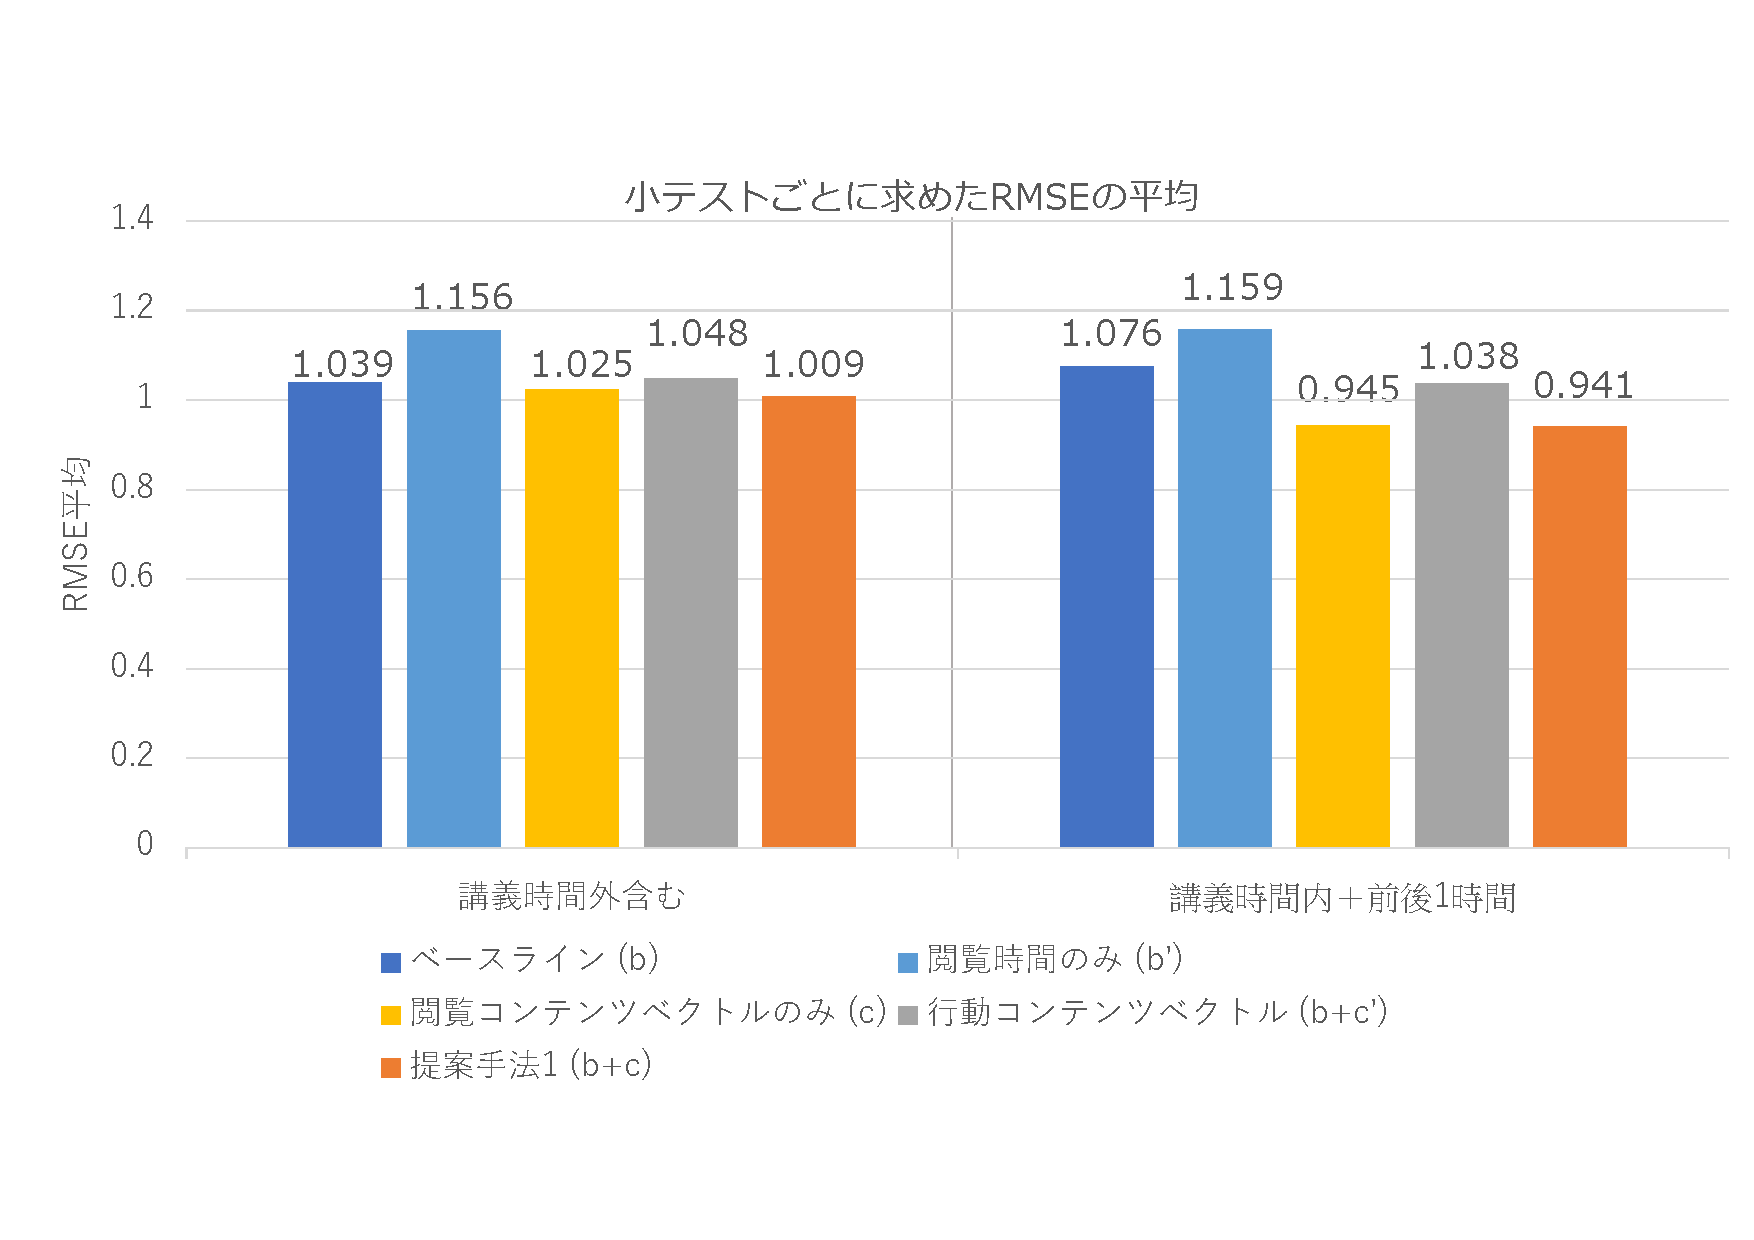
\includegraphics[scale = 0.4]{RMSE_5.pdf}
  \vspace{-10mm}
  \caption{小テストごとに求めたRMSEの平均}
  \label{fig:rmse}
\end{figure}


% \begin{table}[tbp]
%   \centering
%   \caption{講義時間外含む}
%   \label{tb:rmse_each_soto}
%   \begin{tabular}{c||c|c|c|c}
%     小テスト & ベースライン & 閲覧時間のみ & 閲覧コンテンツベクトルのみ & 提案手法1 \\
%     &  (b)  & (b')  &  (c)  &  (b+c)  \\ \hline\hline
%     1週目 & 1.144 & 1.167 & 1.219 & 1.217 \\ \hline
%     2週目 (1)  & 1.052 & 0.975 & 1.166 & 1.083 \\ \hline
%     2週目 (2)  & 1.088 & 1.110 & 0.777 & 0.796 \\ \hline
%     3週目 & 0.909 & 0.867 & 0.619 & 0.611 \\ \hline
%     4週目 & 1.191 & 1.243 & 1.109 & 1.107 \\ \hline
%     5週目 & 1.220 & 1.242 & 0.932 & 0.968 \\ \hline
%     6週目 & 1.075 & 1.229 & 1.199 & 1.132 \\ \hline
%     7週目 & 1.372 & 1.418 & 1.180 & 1.155 \\ \hline\hline
%     平均 & 1.039 & 1.156 & 1.025 & 1.009 \\ \hline
%   \end{tabular}
% \end{table}

% \begin{table}[tbp]
%   \centering
%   \caption{講義時間内および前後1時間}
%   \label{tb:rmse_each_nai}
%   \begin{tabular}{c||c|c|c|c}
%     小テスト & ベースライン & 閲覧時間のみ & 閲覧コンテンツベクトルのみ & 提案手法1 \\
%     &  (b)  & (b')  &  (c)  &  (b+c)  \\ \hline\hline
%     1週目 & 1.051 & 1.084 & 1.072 & 1.103 \\ \hline
%     2週目 (1)  & 1.194 & 1.167 & 1.060 & 1.080 \\ \hline
%     2週目 (2)  & 1.089 & 1.047 & 0.707 & 0.690 \\ \hline
%     3週目 & 0.902 & 0.903 & 0.384 & 0.390 \\ \hline
%     4週目 & 1.283 & 1.201 & 1.068 & 1.007 \\ \hline
%     5週目 & 1.139 & 1.265 & 1.020 & 1.007 \\ \hline
%     6週目 & 1.085 & 1.199 & 1.004 & 0.949 \\ \hline
%     7週目 & 1.433 & 1.407 & 1.242 & 1.233 \\ \hline\hline
%     平均 & 1.076 & 1.159 & 0.945 & 0.941 \\ \hline
%   \end{tabular}
% \end{table}

% 表はマージンにはみ出ているので,おさまるようにしましょう.かつある程度同じぐらいの幅でそろえたい.
% \begin{description}[labelwidth=16em]
%  \item[行動特徴ベクトル(ベースライン)(b)] ページごとに各学生の行動を数えたベクトル$\bm{u}^{(i)}_c$
%  \item[閲覧時間のみ(b')] 各ページの閲覧時間$t^{(i)}_{(c,p)}$を要素としたベクトル
%  \item[閲覧コンテンツベクトル(c)] 各ページベクトルに重みづけしたベクトル$\bm{v}^{(i)}_c$
%  \item[行動コンテンツベクトル(b+c')] コンテンツごとに求めたページベクトルの合計を\\ \hspace{47mm} 行動特徴ベクトル$\bm{u}^{(i)}_c$に連結したベクトル$\bm{C}^{(i)}_c$
% \end{description}
\begin{table}[tbp]
  \centering
  \caption{小テストごとのRMSE(講義時間外含む)}
  \label{tb:rmse_each_soto}
  \begin{tabular}{l||c|c|c|c|c}
    % 小テスト & ベースライン & 閲覧時間のみ & 閲覧コンテンツ & 行動コンテンツ & 提案手法1 \\
    % & (b) & (b') & ベクトル(c) & ベクトル(b+c') & (b+c) \\ \hline\hline
    小テスト & b & b' & c & b+c' & b+c \\ \hline\hline
    % 小テスト & $\bm{u}^{(i)}_c$(b) & $t^{(i)}_{(c,p)}$(b') & $\bm{v}^{(i)}_c$(c) & $\bm{C}^{(i)}_c$(b+c') & (b+c) \\ \hline\hline
    1週目 & 1.144 & 1.167 & 1.219 & 1.158 & 1.217 \\ \hline
    2週目(1)  & 1.052 & 0.975 & 1.166 & 1.166 & 1.083 \\ \hline
    2週目(2)  & 1.088 & 1.110 & 0.777 & 0.887 & 0.796 \\ \hline
    3週目 & 0.909 & 0.867 & 0.619 & 0.611 & 0.611 \\ \hline
    4週目 & 1.191 & 1.243 & 1.109 & 1.181 & 1.107 \\ \hline
    5週目 & 1.220 & 1.242 & 0.932 & 1.000 & 0.968 \\ \hline
    6週目 & 1.075 & 1.229 & 1.199 & 1.094 & 1.132 \\ \hline
    7週目 & 1.372 & 1.418 & 1.180 & 1.284 & 1.155 \\ \hline\hline
    平均 & 1.039 & 1.156 & 1.025 & 1.048 & 1.009 \\ \hline
  \end{tabular}
\end{table}

\begin{table}[tbp]
  \centering
  \caption{小テストごとのRMSE(講義時間内および前後1時間)}
  \label{tb:rmse_each_nai}
  \begin{tabular}{l||c|c|c|c|c}
    % 小テスト & ベースライン & 閲覧時間のみ & 閲覧コンテンツ & 行動コンテンツ & 提案手法1 \\
    % & (b) & (b') & ベクトル(c) & ベクトル(b+c') & (b+c) \\ \hline\hline
    % 小テスト & ベースライン & 閲覧時間のみ & 閲覧 & 行動 & 提案手法1 \\
    % &  &  & コンテンツ & コンテンツ &  \\
    % & (b) & (b') & ベクトル(c) & ベクトル(b+c') & (b+c) \\ \hline\hline
    小テスト & b & b' & c & b+c' & b+c \\ \hline\hline
    1週目 & 1.051 & 1.084 & 1.072 & 1.165 & 1.103 \\ \hline
    2週目(1)  & 1.194 & 1.167 & 1.060 & 1.084 & 1.080 \\ \hline
    2週目(2)  & 1.089 & 1.047 & 0.707 & 0.896 & 0.690 \\ \hline
    3週目 & 0.902 & 0.903 & 0.384 & 0.633 & 0.390 \\ \hline
    4週目 & 1.283 & 1.201 & 1.068 & 1.272 & 1.007 \\ \hline
    5週目 & 1.139 & 1.265 & 1.020 & 1.004 & 1.007 \\ \hline
    6週目 & 1.085 & 1.199 & 1.004 & 0.942 & 0.949 \\ \hline
    7週目 & 1.433 & 1.407 & 1.242 & 1.306 & 1.233 \\ \hline\hline
    平均 & 1.076 & 1.159 & 0.945 & 1.038 & 0.941 \\ \hline
  \end{tabular}
\end{table}


\section{提案手法2}\label{sec:kekka2}

\subsection{スコア予測結果}
提案手法2の結果を図~\ref{fig:rmse_2}に示す.ベースライン,提案手法1と比較するため,それぞれの結果も示している.小テストごとのRMSEの値は表~\ref{tb:rmse_each_soto2},表~\ref{tb:rmse_each_nai2}の通りであり,表~\ref{tb:rmse_each_soto2}は講義時間外の操作を全て用いる場合,表~\ref{tb:rmse_each_nai2}は講義時間内および前後1時間の操作に絞った場合である.

図~\ref{fig:rmse_2}より,講義時間外の行動を含めた場合と講義時間内および前後1時間の行動に絞った場合のどちらの条件でも,小テストと関係のあるページの行動を重要として予測する手法(提案手法2)はベースライン,提案手法1と比べて,RMSEの平均が悪くなった.
% 予測誤差が大きくなった.
提案手法2で講義時間外の行動を含めた場合と講義時間内および前後1時間の行動に絞った場合の比較をすると,講義時間外の行動を含めた場合の方がRMSEの平均が小さく,予測精度がよかった.

小テストごとの結果をみると,講義時間外の行動を含めて予測した場合では,表~\ref{tb:rmse_each_soto}より,1週目がベースライン,2週目(1),3週目,4週目,5週目が提案手法1,2週目(1),6週目,7週目が提案手法2において最もRMSEの平均が小さく,予測精度がよくなった.
% 予測誤差が小さくなった.
講義時間内および前後1時間の行動に絞って予測した場合では,表~\ref{tb:rmse_each_nai}より,1週目がベースライン,2週目(1),3週目,4週目,5週目,6週目,7週目が提案手法1において最もRMSEの平均が小さく,予測精度がよくなった.

\subsection{考察}
提案手法2ではベースラインと比較して,RMSEの平均が大きく,予測精度が悪くなった.加えて,提案手法1では学生の行動を時間で絞ることで予測精度が向上したが,提案手法2では,ベースラインよりも予測精度が悪くなった.
% 予測精度が低下した.
% 「低下」という場合は「ある値からもっと悪い値になった」ことを言うが,提案手法2はここで初めて出てきているので,低下とは言わない.「ベースラインよりも予測誤差が大きい.」など
% これは,提案手法2では全ての学生に対して同じ値を重要度として与えているため,学生間の変化に対応していないからであると考える.
これは,提案手法2ではコンテンツ情報が直接的に使用されていないからであると考える.
% ここはよくわからない.ここの「重要度」とは何でしょう?重要なページに対応する各学生の行動ベクトルを使うので,学生間の変化は出ているのでは?<-確かに
% むしろ「コンテンツ情報」が直接的に使われていないことも理由として考えられそう.(手法1+手法2がもっといいのかもしれませんが)


\begin{figure}[tbp]
  \centering
  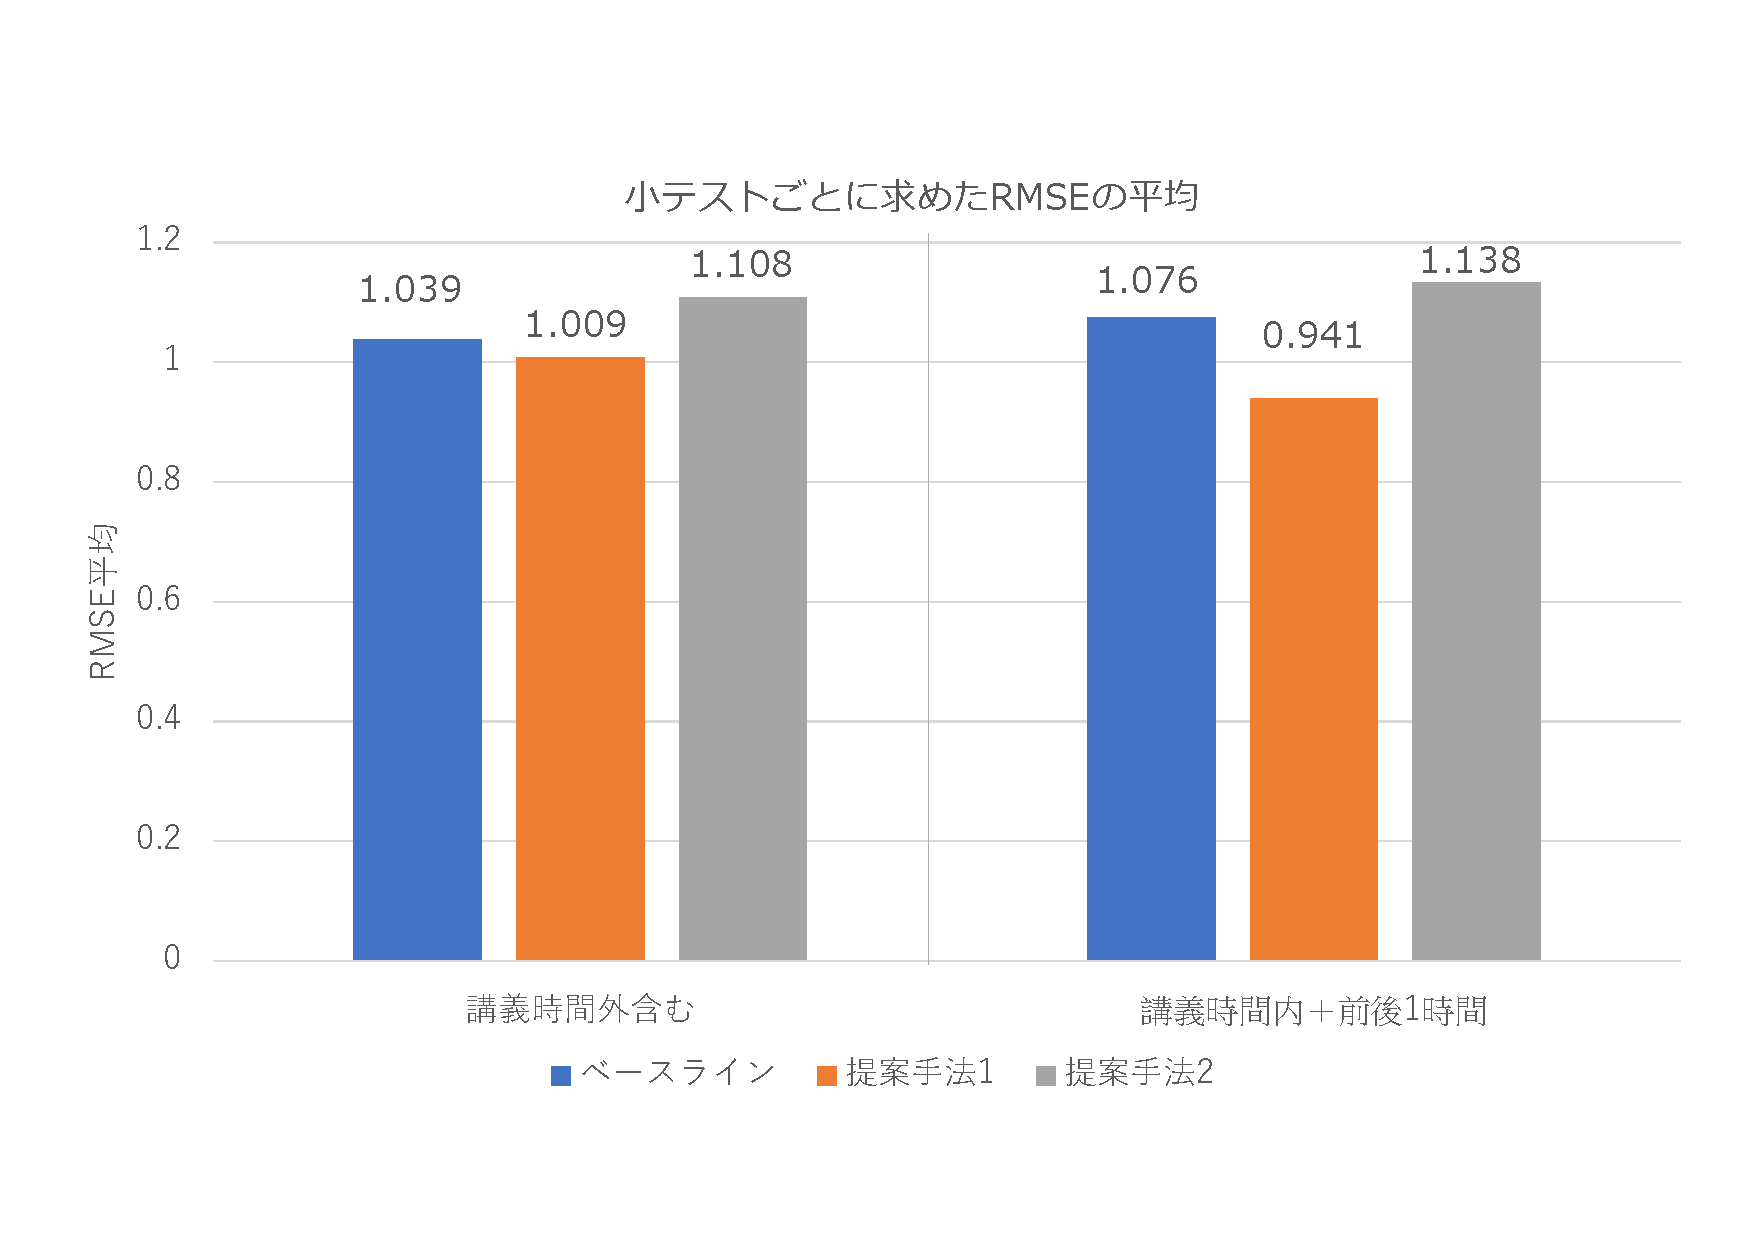
\includegraphics[scale = 0.4]{RMSE_3.pdf}
  \vspace{-10mm}
  \caption{小テストごとに求めたRMSEの平均}
  \label{fig:rmse_2}
\end{figure}

\begin{table}[tbp]
  \centering
  \caption{小テストごとのRMSE(講義時間外含む)}
  \label{tb:rmse_each_soto2}
  \begin{tabular}{l||c|c|c}
    小テスト & ベースライン & 提案手法1 & 提案手法2 \\ \hline\hline
    1週目 & 1.051 & 1.217 & 1.105 \\ \hline
    2週目(1)  & 1.194 & 1.083 & 1.002 \\ \hline
    2週目(2)  & 1.089 & 0.796 & 1.044 \\ \hline
    3週目 & 0.902 & 0.611 & 0.879 \\ \hline
    4週目 & 1.283 & 1.107 & 1.189 \\ \hline
    5週目 & 1.139 & 0.968 & 1.212 \\ \hline
    6週目 & 1.085 & 1.132 & 1.059 \\ \hline
    7週目 & 1.433 & 1.155 & 1.372 \\ \hline\hline
    平均 & 1.076 & 1.009 & 1.108 \\ \hline
  \end{tabular}
\end{table}

\begin{table}[tbp]
  \centering
  \caption{小テストごとのRMSE(講義時間内および前後1時間)}
  \label{tb:rmse_each_nai2}
  \begin{tabular}{l||c|c|c}
    小テスト & ベースライン & 提案手法1 & 提案手法2 \\ \hline\hline
    1週目 & 1.051 & 1.103 & 1.066 \\ \hline
    2週目(1)  & 1.194 & 1.080 & 1.197 \\ \hline
    2週目(2)  & 1.089 & 0.690 & 1.072 \\ \hline
    3週目 & 0.902 & 0.390 & 0.853 \\ \hline
    4週目 & 1.283 & 1.007 & 1.229 \\ \hline
    5週目 & 1.139 & 1.007 & 1.137 \\ \hline
    6週目 & 1.085 & 0.949 & 1.087 \\ \hline
    7週目 & 1.433 & 1.233 & 1.428 \\ \hline\hline
    平均 & 1.076 & 0.941 & 1.134 \\ \hline
  \end{tabular}
\end{table}

% 行動を絞る閾値となる時間を5分ではなく17分,10分と変化させて手法1の予測を行った結果を表に示す?付録にでもかいていいかなあ


\chapter{結論}

本研究は,学習者の行動ログから得られる情報だけでなく,講義資料のコンテンツ情報も用いることで,小テストのスコア予測の精度向上を図ることを目的としている.
% 学生の行動から得られる情報にコンテンツ情報を含めることでの学生が行う小テストのスコア予測の精度向上を目的としている.
% ・「含める」は気になる.直接的に含めたのは手法1だけなので.
% ・「学生」と「学習者」が1文内で混在.
% 「学習者の行動ログから得られる情報だけでなく,講義資料のコンテンツ情報も用いることで,小テストのスコア予測の精度向上を図ることを目的としている」
コンテンツの使用がスコア予測の精度向上に繋がるのか,コンテンツに含まれるテキスト情報のベクトル化を行い,段階的に特徴ベクトルを使用することで検証した.
% 結論では,この研究では何を明らかにしようとしていたかを再度述べたうえで,結果的に何が明らかになったのかについて結論づけてください.(他の論文の結論やConclusionも参考に)
この結果から,コンテンツ情報をスコア予測に用いることは有効であると考える.さらに,学生が長く閲覧したコンテンツ情報を用いることが,スコア予測の精度向上に繋がる可能性があることが示された.
% さらに,コンテンツ情報だけではなく,学生の行動から重要度を求め,スコア予測に使用することは,スコア予測の精度向上に繋がる可能性があることが示された.

今後の課題として以下のものが挙げられる.

\begin{description}

 \item[ページベクトルの計算方法]
ページベクトルに関して,本研究ではページに含まれるテキスト情報のみをベクトル化したが,ページ内の図表の位置関係,および図に含まれる文字も同様にベクトル化を行い,ページベクトルの要素とすることができれば,ページの情報を深く取得することになり,より高い精度が期待できる.

 \item[ページ重要度の計算方法]
提案手法2では,ベースラインに比べ予測精度は低くなっているが,ページの重要度の求め方を変えることによって,予測精度が上がる可能性がある.具体的には,教師が長く説明したページほど重要度を高く設定する,学生の操作回数が多いページほど重要度を高く設定するなどである.
% 提案手法2は十分に取り組むことができなかっため,今後検討していきたい.

 \item[特徴量に対する重要度の利用]
提案手法1では閲覧時間を重要度として特徴量に加え,提案手法2では小テストとの関係をページの重要度として特徴量に加えた.ここで二つの手法より,ページの重要度に加え,閲覧時間以外の行動の重要度をLightGBMで求めたImportanceに沿って変えることで,予測に必要な情報が厳選され,より高い精度を期待できる.

 \item[ベクトルの次元数]
本研究で使用した閲覧コンテンツベクトル,行動特徴ベクトルは使用する行動を削る以外の方法で次元数削減を行っていないため,高い次元数のまま予測を行っている.しかし,次元数を落とすことで予測精度が変化する可能性があるため,次元削減の手法を検討する必要がある.

 \item[予測結果についての考察]
~\ref{sec:kekka1}節の結果について,何が各週の予測結果の違いに影響を及ぼしているのかを十分に検証できていないため,今後の課題となる.

% 追加
 \item[理解度予測]
本論文では小テストごとに5点満点の点数予測を行ったが,1問ごとに正解/不正解の予測を行うことで,より深い学生の理解度予測に繋がる可能性がある.


\end{description}
% 結果の違いがどこからでているか (実際のコンテンツでどういう違いがあるからこういう差が生まれているのか) って具体的に書いていいもの?
% まあ文章が多い/図が多い/具体例が多い程度ならいいのかな総合的に見てどういう差になっているかということ


\vspace{2mm}
\chapter*{謝辞}

本研究を行うにあたり,川嶋教授には研究のアイデアをいただき,また,研究,論文執筆に関して多大なる有益な助言をいただき,大変お世話になりました.深く感謝申し上げます.

九州大学島田教授,峰松准教授にはデータの提供,また,研究,論文への助言をいただきました.深く感謝申し上げます。

最後に,川嶋研究室の皆様には普段から研究に関してご助言,ご協力いただきました.本当にありがとうございました。


% 参考文献
% {
% \footnotesize
\bibliography{sotsuronkogishi}
\bibliographystyle{junsrt}
% }

\appendix
\chapter{付録}
\section{各小テストのトピック}
表~\ref{tb:topic}は各小テストに対応するコンテンツのページ数である.1週目は2つのコンテンツが使用されているため,表のような記載となっている.

\begin{table}[tbp]
  \centering
  \caption{各小テストに対応するコンテンツのページ数}
  \label{tb:topic}
  \begin{tabular}{l||c}
    小テスト & ページ数 \\ \hline\hline
    1週目 & 8+13 \\ \hline
    2週目(1) & 66 \\ \hline
    2週目(2) & 62 \\ \hline
    3週目 & 30 \\ \hline
    4週目 & 49 \\ \hline
    5週目 & 29 \\ \hline
    6週目 & 46 \\ \hline
    7週目 & 82 \\ \hline
  \end{tabular}
\end{table}

% 各週でImportance見た時の結果もだしたい
% ↑Importanceでわりと特徴が違うから予測結果の違いに関わっているかも

\end{document}



